\documentclass[12pt, reqno]{amsbook}
%
\usepackage{eurosym}
\usepackage{amsmath}
\usepackage{amssymb}
\usepackage{amsfonts}
\usepackage[onehalfspacing]{setspace}
\usepackage{chngcntr}
\usepackage{graphicx}
\usepackage[a4paper, margin=2.5cm]{geometry}
\usepackage[english]{babel}
\usepackage{fancyhdr}
\usepackage{titlesec}
\usepackage{enumitem}
\usepackage{etoolbox}
\usepackage{csquotes}
\usepackage{url}
\usepackage{placeins}
\usepackage[printonlyused]{acronym}
\usepackage{float}
\usepackage{booktabs}
\usepackage{array}
\usepackage{longtable}

%
% Uncomment the command below if you use eps format for figures
%\usepackage{epstopdf}
%

\usepackage[
    backend=biber,
    style=numeric,
    sorting=none,
  ]{biblatex}
\addbibresource{references.bib}

\usepackage{hyperref}
\usepackage{xcolor}
%\hypersetup{colorlinks, linkcolor={blue!50!black}, citecolor={blue!50!red}, urlcolor={blue!80!black}}
\hypersetup{colorlinks, linkcolor=black, citecolor=black, urlcolor=black}

\titleformat{\subsubsection}{\normalfont\normalsize\bfseries}{\thesubsubsection}{0.5em}{}
\titlespacing*{\subsubsection} {0pt}{2.25ex plus 1ex minus .2ex}{1.5ex plus .2ex}

\makeatletter
\def\l@subsection{\@tocline{2}{0pt}{2.5pc}{5pc}{}}
%\def\l@subsubsection{\@tocline{2}{0pt}{5pc}{7.5pc}{}}
\makeatother

\makeatletter
\def\subsubsection{\@startsection{subsubsection}{3}%
  \z@{.5\linespacing\@plus.7\linespacing}{.1\linespacing}%
  {\normalfont\itshape}}
\makeatother

\makeatletter
    \def\section{\@startsection{section}{1}%
      \z@{.5\linespacing\@plus.7\linespacing}{.25\linespacing}%
      {\normalfont\bfseries\flushleft}}
    \def\subsection{\@startsection{subsection}{2}%
      \z@{.5\linespacing\@plus.7\linespacing}{.25\linespacing}%
      {\normalfont\bfseries\flushleft}}
\makeatother
\setcounter{MaxMatrixCols}{10}
%
\providecommand{\U}[1]{\protect\rule{.1in}{.1in}}
\theoremstyle{definition}

\usepackage{amsthm}

\theoremstyle{definition}
\newtheorem*{hypothesis}{Hypothesis}
\newtheorem*{research_question}{Research Question}
\newtheorem{requirement}{Requirement}
%
\makeatletter
\newcommand\frontFont{\@setfontsize\frontFont{14.4}{14.4}}
\newcommand\numberprefix{}
\def\numberline#1{\hb@xt@\@tempdima{\numberprefix #1\hfil}}
\def\l@figure#1#2{\@tocline{0}{3pt plus2pt}{0pt}{6pc}{}%
  {\renewcommand\numberprefix{Figure~}#1}{#2}}
\def\l@table#1#2{\@tocline{0}{3pt plus2pt}{0pt}{6pc}{}%
  {\renewcommand\numberprefix{Table~}#1}{#2}}
\makeatother
%
% Please write the references according to your school
%
\newenvironment{dedication}
  {%\clearpage           % we want a new page
   \thispagestyle{empty}% no header and footer
   \vspace*{\stretch{1}}% some space at the top
   \itshape             % the text is in italics
   \raggedleft          % flush to the right margin
  }
  {\par % end the paragraph
   \vspace{\stretch{3}} % space at bottom is three times that at the top
   %\clearpage           % finish off the page
  }
  \numberwithin{section}{chapter}
\fancyhead{}
\fancyfoot{}
\pagestyle{fancy}
\fancyfoot[R]{\thepage} % Before oneside: \fancyfoot[LE,RO]{\thepage}
%
\makeatletter
\def\ps@plain{\ps@empty
 \def\@evenfoot{%
   \normalfont\scriptsize
   \rlap{\thepage}\hfil
   }%
 \def\@oddfoot{%
   \normalfont\scriptsize \hfil
   \llap{\thepage}}%
}
\makeatother
\renewcommand{\headrulewidth}{0pt}
\renewcommand{\footrulewidth}{0pt}
%
\usepackage{montserrat}
\usepackage[T1]{fontenc}
\renewcommand*\oldstylenums[1]{{\fontfamily{Montserrat-TOsF}\selectfont #1}}
%
\numberwithin{table}{chapter}
\numberwithin{figure}{chapter}
\newcolumntype{M}[1]{>{\centering\arraybackslash}m{#1}}
\definecolor{MyDarkBlue}{rgb}{0,0.08,0.45}
\makeatletter
\def\cleardoublepage{\clearpage\if@twoside%
  \ifodd\c@page\else
  \vspace*{\fill}
  \hfill
  \begin{center}
  {\fontfamily{Montserrat-TOsF}\selectfont\small [ This page is intentionally left blank. ]}

  \end{center}
  \vspace{\fill}
  \thispagestyle{empty}
  \newpage
 \if@twocolumn\hbox{}\newpage\fi\fi\fi
}
\makeatother
%
%
% Avoids the indentation of the first paragraph
%
\makeatletter
\let\@afterindenttrue\@afterindentfalse
\makeatother
%

\raggedbottom
\begin{document}

\sffamily
\frontFont
\begin{flushleft}
  
\includegraphics[width=6.03cm]{images/iscte}\\[3.3mm]

  %\hrulefill
  \textcolor{MyDarkBlue}{\rule {14.9cm} {1pt}}
  ~\\
  ~\\
  ~\\
  \textbf{Design and Evaluation of a Cloud-Native Web API for Third-Party Integrations}
  ~\\
  ~\\
  ~\\
  ~\\
  Rafael Bruce Tomé Santos\\
  ~\\
  ~\\
  ~\\
  Master in Computer Engineering\\
  ~\\
  ~\\
  ~\\
  Supervisors:\\
  ~\\
  Doctor Ana Maria de Almeida, Associate Professor,\\
  Iscte -- Instituto Universitário de Lisboa\\
  ~\\
  Doctor Carlos Coutinho, Assistant Professor,\\
  Iscte -- Instituto Universitário de Lisboa\\
  ~\\
  ~\\
  ~\\
  ~\\
  September, 2025
\end{flushleft}
\thispagestyle{empty}

\cleardoublepage

\begin{flushleft}
  
\includegraphics[width=6.03cm]{images/ista}\\[7mm]
  \textcolor{MyDarkBlue}{\rule {14.9cm} {1pt}}
  ~\\
  ~\\
  ~\\
  Department of Information Science and Technology\\
  ~\\
  ~\\
  \textbf{Design and Evaluation of a Cloud-Native Web API for Third-Party Integrations}\\
  ~\\
  ~\\
  ~\\
  ~\\
  Rafael Bruce Tomé Santos\\
  ~\\
  ~\\
  ~\\
  Master in Computer Engineering\\
  ~\\
  ~\\
  ~\\
  Supervisors:\\
  ~\\
  Doctor Ana Maria de Almeida, Associate Professor,\\
  Iscte -- Instituto Universitário de Lisboa\\
  ~\\
  Doctor Carlos Coutinho, Assistant Professor,\\
  Iscte -- Instituto Universitário de Lisboa\\
  ~\\
  ~\\
  ~\\
  ~\\
  September, 2025
\end{flushleft}
\thispagestyle{empty}
\rmfamily
\normalsize
\frontmatter
\thispagestyle{empty}

\frontmatter
\addtocontents{toc}{\setcounter{tocdepth}{2}}
\thispagestyle{empty}

\setcounter{page}{1}
\pagenumbering{roman} %
\chapter*{Acknowledgment}

This dissertation represents an end to a long academic journey. I am grateful for my family and friends, who gave me their unconditional support throughout this time. I want to give a special tribute to my father, who I know would be very proud of this achievement. I would also like to thank my supervisors, Doctor Ana Maria de Almeida and Doctor Carlos Coutinho, for their guidance and patience.

\chapter*{Resumo}

Escrever aqui o resumo em Português.

\vspace{3ex}
\textsc{Palavras Chave:} \textit{palavra\_1}, \textit{palavra\_2}, \dots

\chapter*{Abstract}

Write your abstract here in English.

\vspace{3ex}
\textsc{Keywords:} \textit{word\_1}, \textit{word\_2}, \dots

\tableofcontents
\listoffigures
\listoftables
\cleardoublepage
%\printglossary[type=\acronymtype, nonumberlist, nogroupskip]
\chapter*{List of Acronyms}
\begin{acronym}
  \acro{AI}{Artificial Intelligence}
  \acro{API}{Application Programming Interface}
  \acro{AWS}{Amazon Web Services}
  \acro{CI/CD}{Continuous Integration/Continuous Delivery}
  \acro{CORS}{Cross-Origin Resource Sharing}
  \acro{CPU}{Central Processing Unit}
  \acro{CRUD}{Create Read Update Delete}
  \acro{DNS}{Domain Name System}
  \acro{DSRM}{Design Science Research Methodology}
  \acro{DTO}{Data Transfer Object}
  \acro{ECS}{Elastic Container Service}
  \acro{GB}{Gigabyte}
  \acro{GiB}{Gibibyte}
  \acro{GCP}{Google Cloud Platform}
  \acro{HTTP}{Hypertext Transfer Protocol}
  \acro{HTTPS}{Hypertext Transfer Protocol Secure}
  \acro{IaC}{Infrastructure as Code}
  \acro{IATA}{International Air Transport Association}
  \acro{IaaS}{Infrastructure as a Service}
  \acro{IDE}{Integrated Development Environment}
  \acro{IT}{Information Technology}
  \acro{I/O}{Input/Output}
  \acro{IS}{Information System}
  \acro{JSON}{JavaScript Object Notation}
  \acro{JWT}{JSON Web Token}
  \acro{KB}{Kilobyte}
  \acro{LCL}{Less than Container Loaded}
  \acro{OAuth}{Open Authorization}
  \acro{OIDC}{OpenID Connect}
  \acro{ORM}{Object Relational Mapping}
  \acro{OS}{Operating System}
  \acro{PaaS}{Platform as a Service}
  \acro{PRISMA}{Preferred Reporting Items for Systematic reviews and Meta-Analyses}
  \acro{RBAC}{Role-Based Access Control}
  \acro{RDS}{Relational Database Service}
  \acro{REST}{Representational State Transfer}
  \acro{RPC}{Remote Procedure Call}
  \acro{SaaS}{Software as a Service}
  \acro{SOA}{Service-Oriented Architecture}
  \acro{SPA}{Single-Page Application}
  \acro{SQL}{Structured Query Language}
  \acro{UI}{User Interface}
  \acro{URL}{Uniform Resource Locator}
  \acro{vCPU}{Virtual Central Processing Unit}
  \acro{VNet}{Virtual Network}
  \acro{VM}{Virtual Machine}
  \acro{XML}{eXtensible Markup Language}
\end{acronym}

\mainmatter

\hyphenation{wri-te he-re pro-per hy-phe-ni-za-tion}

\setcounter{page}{1} \pagenumbering{arabic}
\acresetall

\chapter{Introduction}
\label{Chapter:Introduction}

\section{Context}
\label{Section:Context}

Digital transformation is changing the way businesses communicate with a network of partners and third-party service providers. This shift is powered by \acp{API}, which enable software systems to communicate with each other smoothly~\cite{Hunturu2023}. However, this increased connectivity fuels the need to aggregate and integrate heterogeneous external services into a unified platform. Companies seeking to build platforms must often interact with several third-party \acp{API} that vary widely in their design, data formats, communication protocols, and reliability. This inconsistency creates complexity, making it more difficult to build systems that are scalable, maintainable, and resilient~\cite{Huf2019}.

The freight forwarding industry serves as a case study for this integration challenge. Many companies in this industry are undergoing digitalization to meet growing client demands and remain competitive~\cite{Wang2021}. Traditional freight forwarders have been lagging behind due to an overreliance on manual processes. This gives rise to digital freight forwarders that provide more advanced and automated services, integrating several carrier providers, often across multiple modes of transport~\cite{Sullivan2021}.

Devlop\footnote{Devlop, \url{https://devlop.systems/}, (accessed 16 Aug. 2025)}, an \acp{IS} company from Portugal that specializes in developing solutions for the transport and logistics sectors, proposed creating a web application to provide real-time freight quotes from multiple carriers to customers. To this effect, two external \acp{API} would be integrated: WebCargo\footnote{WebCargo, \url{https://www.webcargo.co/about/}, (accessed 19 Aug. 2025)} (for air transport) and Cargofive\footnote{Cargofive, \url{https://cargofive.com/}, (accessed 19 Aug. 2025)} (for sea transport). A traditional monolithic software architecture is not suitable for this as the application grows, since an issue in one integration could hinder the entire system. This establishes the need for a more robust and scalable approach.

This dissertation proposes a conceptual framework to address these integration and scalability challenges, which may be present in other projects with similar characteristics in any industry. To do so, it uses a proof-of-concept implementation that applies a microservice-based architecture and is hosted on a remote cloud platform.

\section{Motivation}
\label{Section:Motivation}

The dissertation aims to address the architectural challenges faced when integrating various third-party \acp{API} by investigating a cloud-native microservices approach. The application proposed by Devlop faces these difficulties. The development of effective and scalable software is crucial to the success of modern freight forwarding digital platforms, especially in a time when choosing the right technology to address all user requirements is becoming more difficult~\cite{Mushica2024}.

Even though the theoretical benefits of microservices and cloud computing are well-documented in scientific literature, there is a lack of practical case studies. The few studies that go beyond theory tend to focus on specific and isolated architectural features rather than presenting a complete framework for building an entire application. This work moves the discussion from theoretical advantages to a complete implementation, providing a concrete case study to the field of software architecture.

\section{Research Questions}
\label{Section:Research_Questions}

Based on the considerations presented in Section~\ref{Section:Motivation}, this research presents a conceptual framework for developing cloud-native web \acp{API} that integrate and aggregate external services. This study is guided by this research question:

\begin{research_question}
  How to design and implement a software architecture that meets the requirements of complex web applications integrating several external \acp{API}?
\end{research_question}

The research question leads the following hypothesis, which will be studied in this paper:

\begin{hypothesis}
  A microservices architecture, orchestrated through an \ac{API} Gateway and deployed to a cloud platform, is the most suitable choice for complex web applications integrating multiple external \acp{API}.
\end{hypothesis}

\section{Research Methodology}
\label{Section:Research_Methodology}

This dissertation follows the \ac{DSRM}, a six-step research approach often used to create \ac{IS}-related artifacts such as models, methods, design theories, or, in this context, an instantiation~\cite{Peffers2007}.

This dissertation adheres to the "Design \& Development Centered Initiation" entry point shown in Figure \ref{Figure:DSRM}, as the first and second steps have already been presented in Chapter \ref{Chapter:Introduction}.

\begin{figure}[H]
  \centering
  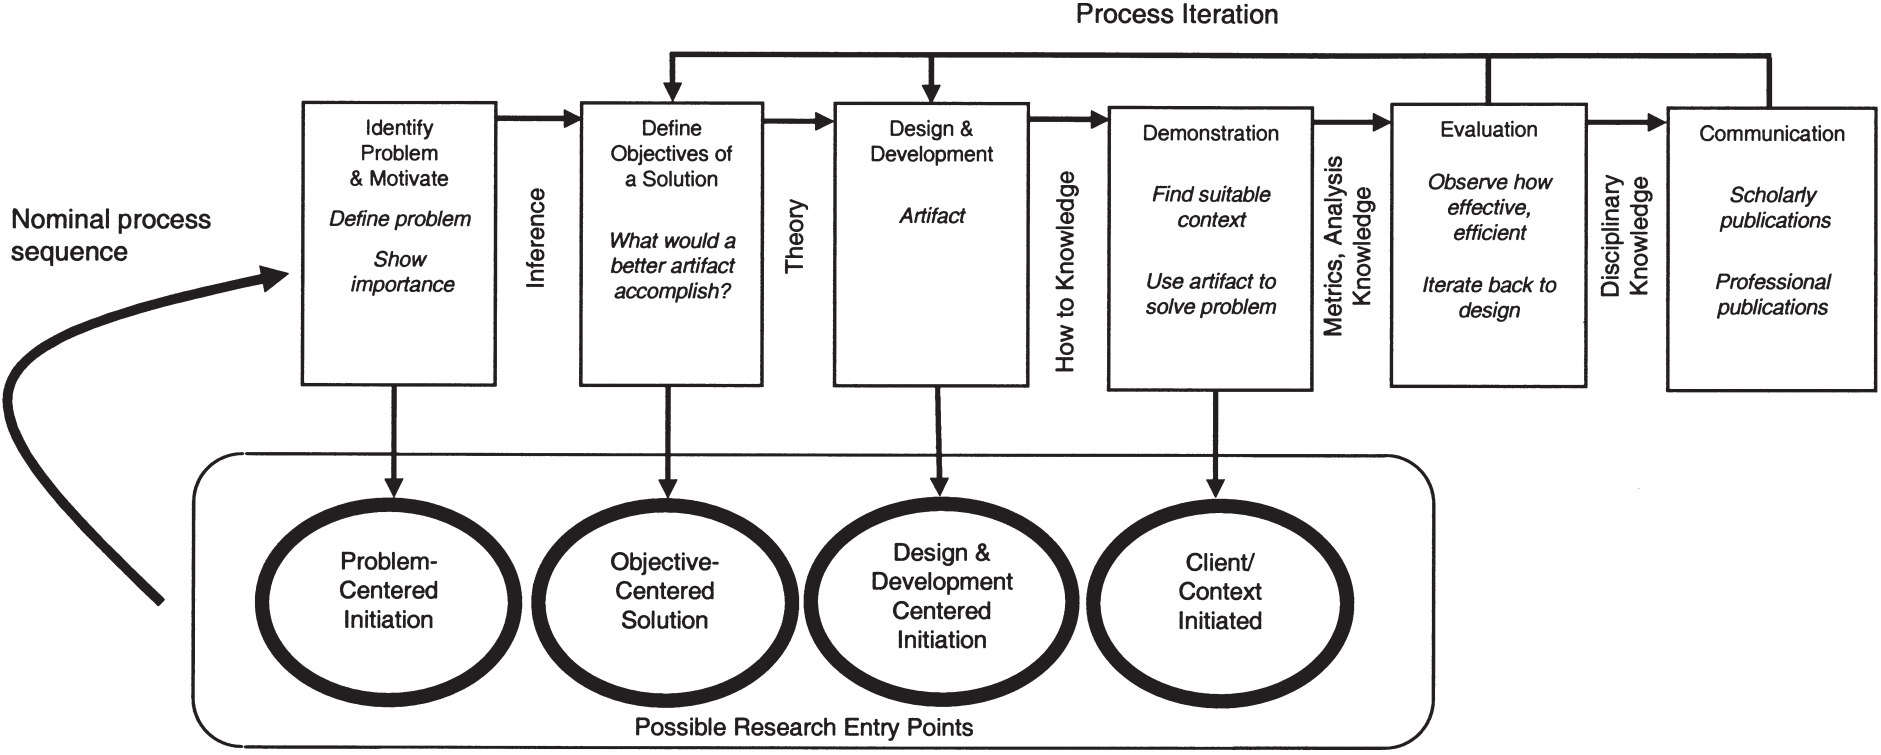
\includegraphics[width=1\linewidth]{images/DSRM_process_model.png}
  \caption{\label{Figure:DSRM}Design Science Research Methodology~\cite{Peffers2007}}
\end{figure}

The following list briefly explains what each step entails and where it is located in this paper:

\begin{description}
  \item [Problem Identification and Motivation] Section \ref{Chapter:Introduction} highlights that despite \acp{API} being crucial for business connectivity, integrating multiple external \acp{API} creates significant challenges for scalability and reliability. A freight forwarding industry project is introduced as a case study. The motivation expressed in Section \ref{Section:Motivation} is to offer a solution to these problems and contribute with a complete case study to the scientific literature.
  \item [Definition of Solution Objectives] The goals of the solution proposed in this dissertation are introduced in Section \ref{Section:Motivation}. In Section \ref{Section:Requirements}, all requirements are precisely listed and defined, further clarifying the objectives of the solution.
  \item [Design and Development] Chapter \ref{Chapter:Design_And_Architecture} details the architecture of the entire solution, while Chapter \ref{Chapter:Implementation} reveals important parts of the implementation process.
  \item [Demonstration] Chapter \ref{Chapter:Implementation} demonstrates a working artifact deployed on a remote cloud.
  \item [Evaluation] Chapter \ref{Chapter:Evaluation} evaluates the developed instantiation considering its reliability, performance, predicted cost, and efficacy.
  \item [Communication] This dissertation itself serves as a means of communication, intended for both academic and business audiences. Chapter \ref{Chapter:Conclusion} summarizes the most relevant findings.
\end{description}

\section{Document Structure}
\label{Section:Document_Structure}

This document is divided into seven chapters.

Chapter \ref{Chapter:Introduction} introduces the context, motivation, research questions, and the research methodology of this dissertation.

Chapter \ref{Chapter:Literature_Search_Methodology} explains the literature search methodology, including the strategy for identifying relevant literature and the papers included in the review.

Chapter \ref{Chapter:Literature_Review} presents a literature review that offers a theoretical background on the main topics relevant to this dissertation.

Chapter \ref{Chapter:Design_And_Architecture} details the design and architecture of the proposed solution.

Chapter \ref{Chapter:Implementation} demonstrates and discusses the implementation of the proposed solution.

Chapter \ref{Chapter:Evaluation} evaluates the implemented solution on correctness, cost, performance, and efficacy.

Chapter \ref{Chapter:Conclusion} concludes the dissertation, highlighting the main findings, limitations, and suggesting future work.


\chapter{Literature Search Methodology}
\label{Chapter:Literature_Search_Methodology}

This chapter describes the methodology used to gather relevant literature for the review presented in Chapter \ref{Chapter:Literature_Review}, along with its results. The search process follows the \ac{PRISMA} guidelines, as explained in Section \ref{Section:PRISMA_S}.

\section{PRISMA-S}
\label{Section:PRISMA_S}

Because \ac{DSRM} does not define a method to search scientific literature, PRISMA-S was used as the basis for the literature search. \ac{PRISMA} is a complete set of guidelines used to improve the reporting of systematic literature reviews, promoting rigor. PRISMA-S (or PRISMA-Search) is a reporting guideline that extends PRISMA, contributing with a detailed checklist specifically for reporting literature search methods.

\section{Information Sources}
\label{Section:Information_Sources}

The b-on\footnote{b-on, \url{https://www.b-on.pt/en/}, (accessed 16 Aug. 2025)} platform was used for the PRISMA-S literature search. b-on is a library that aggregates multiple databases\footnote{b-on, "Collections", \url{https://www.b-on.pt/en/collections/}, (accessed 16 Aug. 2025)}, including IEEE, Web of Science, and Elsevier. This agglomeration removes the need to search individual databases separately.

\section{Search Strategies}
\label{Section:Search_Strategies}

The search was performed using the exact query shown below, where "TI" and "AB" stand for "title" and "abstract", respectively:
\vspace{0.5cm}
\begin{verbatim}
(TI ("web API*" OR "backend*" OR "web application*")
OR AB ("web API*" OR "backend*" OR "web application*"))
AND TI (Architecture OR Develop* OR Design)
AND TI (Cloud* OR Microservice*)
\end{verbatim}
\vspace{0.5cm}

The following search filters were applied in sequence:

\begin{enumerate}
  \item The document must be from 2015 or later.
  \item The document must be peer-reviewed.
  \item The document must be written in English or Portuguese.
\end{enumerate}

\section{Search Results}
\label{Section:Search_Results}

Once the search query was run and all aforementioned filters were applied, all filtered documents went through a process to determine whether they would be included in the final review. That process is shown in Figure \ref{Figure:Literature_Search_Flow_Diagram}.

\begin{figure}[H]
  \centering
  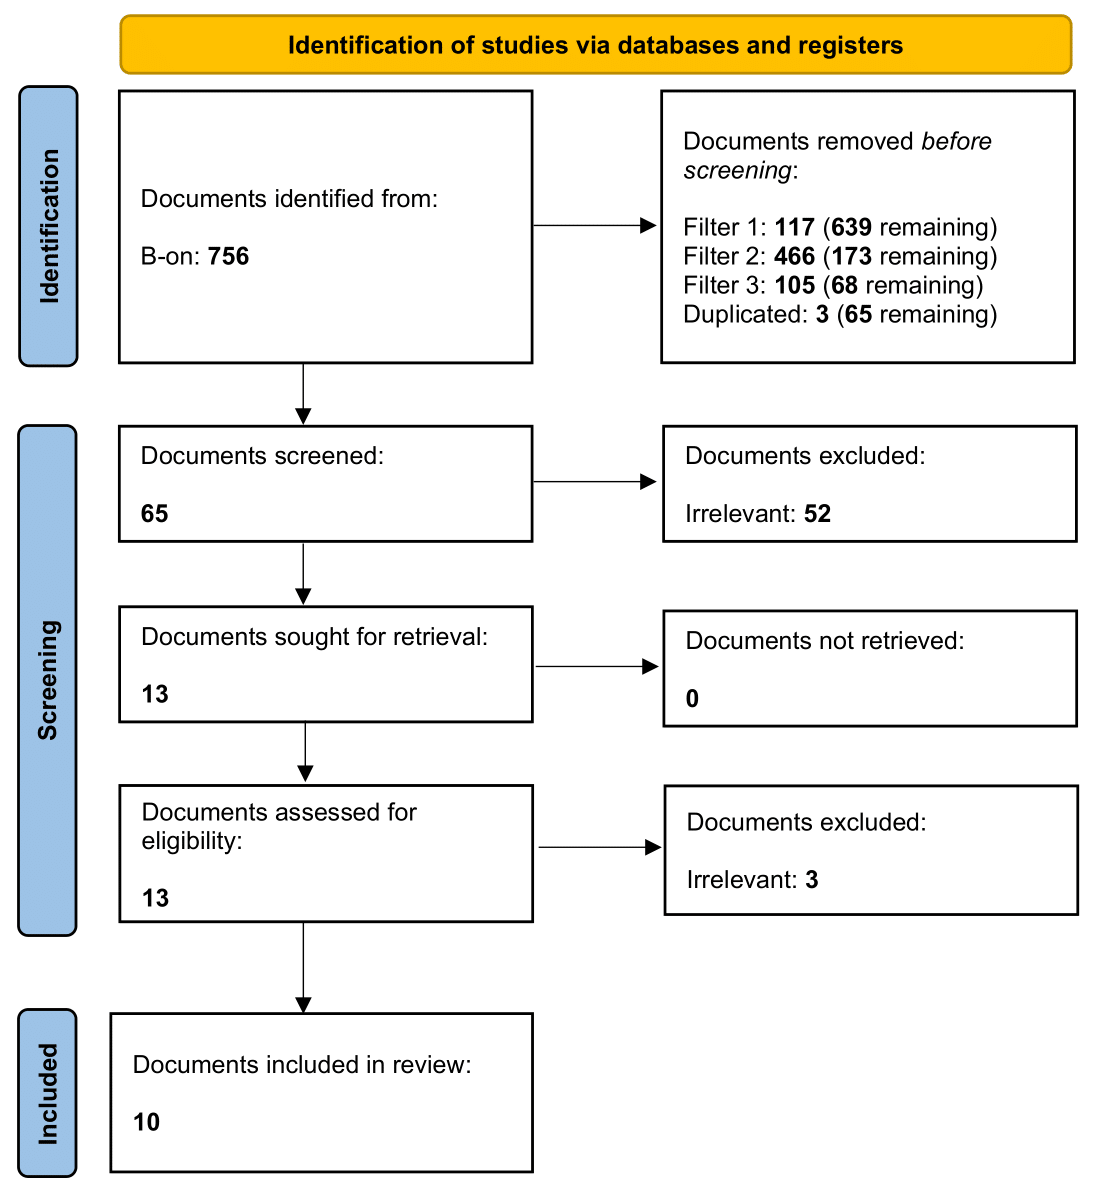
\includegraphics[width=0.9\linewidth]{images/Literature_Search_Flow_Diagram.png}
  \caption{\label{Figure:Literature_Search_Flow_Diagram}Literature Search Flow Diagram}
\end{figure}

The search query identified 756 documents. Upon filtering and deduplication, 65 documents remained. These documents went through a screening process that involved reading their titles and abstracts to determine their relevance. After screening, 13 documents were left. The eligibility of these documents was then evaluated by reading their full text to verify their relevance more rigorously. Only 10 documents were included in the final review, some of which did not present a complete architectural approach for a web \acp{API} or web application. This outcome matches the lack of literature on this topic mentioned in Section \ref{Section:Motivation}.

\section{Further Search}
\label{Section:Further_Search}

The 10 resulting documents gathered in Section \ref{Section:Search_Results} did not offer a comprehensive and varied view of web applications or web \acp{API}. Therefore, additional literature searches were conducted based on topics present in those 10 documents, namely Monolithic and Microservice Architectures, Cloud Computing, Authentication and Authorization, Containerization, and Web \ac{API} Frameworks.

Furthermore, a literature search on freight forwarding was done to better understand the business domain of the web API that will be developed. To perform this further research, b-on, Google Scholar, and websites from authoritative sources were accessed.

\chapter{Literature Review}
\label{Chapter:Literature_Review}

Based on the literature search methodology presented in Chapter \ref{Chapter:Literature_Search_Methodology}, this chapter provides a theoretical background on the main topics relevant to this dissertation.

\section{Freight Transportation Overview}
\label{Section:Freight_Transportation_Overview}

Freight transportation is defined as the flow and storage of goods throughout a supply chain, from an origin to a destination. To achieve this, several stakeholders contribute to the process~\cite{Song2021, Huber2021}. In this project, since the application to develop will be administered by a freight forwarding company, the most important ones are the following:

\begin{description}
  \item [Shipper] The person or company that sells goods to be sent from one location to another. They are the initiators of the whole process, generating the demand for freight transportation~\cite{Song2021}.
  \item [Carrier] The party that provides the transportation service of goods, such as a shipping or airline company~\cite{Song2021}.
  \item [Freight forwarder] The intermediary entity between the shipper and the carriers. It organizes and coordinates the shipment of goods on behalf of its customer seller (the shipper). They are usually responsible for selecting and contracting with appropriate carriers, container consolidation, shipment tracking, transshipment, negotiating delivery terms and freight rates, among other activities~\cite{Song2021, Huang2019}.
\end{description}

\begin{figure}[H]
  \centering
  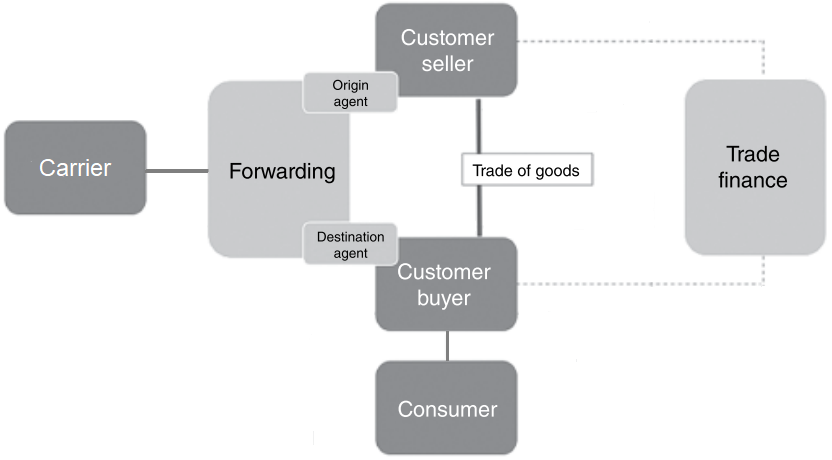
\includegraphics[width=0.9\linewidth]{images/FreightForwarding.png}
  \caption{\label{Figure:FreightForwarding}Freight Forwarding Stakeholders, adapted from~\cite{Peffers2007}}
\end{figure}

Understanding freight rates is relevant for this project, since responding to quotation requests from shippers is one of its goals. The freight rate is the definite cost a carrier charges to transport a specific cargo from one location to another. This cost depends on factors like the cargo's weight, volume, mode of transport, and travel distance. A freight quote is a comprehensive estimate of the total cost to transport a particular cargo from an origin to a destination, which includes the freight rate and any additional fees~\cite{Song2021, Mairon_Freight, Wang2021, WebCargo}.

Various transport modes may be used, including air, sea, waterway, road, and rail. Multiple modes of transport may also be used throughout the journey, a practice known as multimodal transport. In 2019, 70\% of the global freight (measured in tonne-kilometers) was done by ships, followed by road vehicles with 22\%, trains with 7\%, and air vehicles with less than 1\%~\cite{ITF2023}.

Although shippers have the option to work directly with carrier companies, many enterprises, especially small to medium-sized ones, resort to the services provided by freight forwarders. These enterprises tend to deliver \ac{LCL} cargo, which requires consolidation to achieve cost-efficient transportation. The expertise of freight forwarders and their wide network of carriers help shippers find the most appropriate offers and reduce freight rates, decreasing the total delivery price~\cite{Huang2019}.


\section{Web \texorpdfstring{\acp{API}}{API} Overview}
\label{Section:Web_API_Overview}

An \ac{API} is a set of rules and specifications that define how software components or applications should interact with each other. In this dissertation, web \acp{API} are specifically defined as server-side (backend) web \acp{API}, which act as an exposed interface for a web server. They allow client systems like web browsers and mobile applications to interact with the server's resources without needing to know its internal structure and implementation~\cite{Jin2018,Neumann2021, Khozaimi2022}.

Essentially, a web \ac{API} acts as an abstraction layer that facilitates communication through a request-response cycle. A client sends a request to a specific endpoint on a server, which contains details about the desired operation and any necessary data. The server processes the request and returns an \ac{HTTP} response. This response contains a status code indicating success or failure and, depending on the request, a body with the requested data, often formatted in \ac{JSON} or \ac{XML}. This client-server relationship forms a complete web application that end-users can use~\cite{Jin2018,Neumann2021, Khozaimi2022}.

Web \acp{API} specifications come in different architectural styles, which define the syntax and structure of the client-server interactions. These include:

\begin{description}
  \item [\ac{REST}] The most widely used architectural style for \ac{API} development. It organizes its operations around resources, which may be any information that can be identified or named within the context of a web application, such as users, files, purchases, events, etc. \ac{REST} \acp{API} generally use standard \ac{HTTP} methods to perform \ac{CRUD} operations on these resources: "GET" to read, "POST" to create, "PUT" and "PATCH" to update, and "DELETE" to delete~\cite{Neumann2021,Lauret2019, Suryotrisongko2017, Khozaimi2022}.
  \item [GraphQL] This architecture allows clients to specify the exact structure of the data they require. Unlike \ac{REST}, which often requires multiple requests to different endpoints to gather related data (under-fetching) or returns more data than needed (over-fetching), GraphQL exposes a single endpoint. This reduces the amount of data transferred over the network, at the cost of development complexity~\cite{Neumann2021,Lauret2019}.
  \item [\ac{RPC}] \ac{RPC} \acp{API} are function-based, unlike \ac{REST} and GraphQL \acp{API}, which are centered on resources and data, respectively. Each endpoint these \acp{API} expose are associated with a particular function on the server side. This architectural style can offer high performance with its deserialization method, as well as bidirectional and real-time streaming communication support. However, it can be harder for consumers of these \acp{API} to find the desired endpoints, as it is less standardized~\cite{Neumann2021,Lauret2019}.
\end{description}

\section{Web \texorpdfstring{\ac{API}}{API} Security: Authentication and Authorization}
\label{Section:Web_API_Security}

Web \acp{API} expose potentially confidential operations and data, requiring robust security measures. These measures can be understood as two layers: authentication and authorization.
Authentication is the process of identifying users and verifying if they are indeed who they claim to be. Authorization is processed after authentication and determines the actions that a specific user is allowed to perform~\cite{Gupta2024, deAlmeida2022}.

There are several security protocols and mechanisms to address authentication and authorization, including:
\begin{description}
  \item[\ac{OAuth} 2.0] The \ac{OAuth} protocol is an authorization framework that allows users to access backend services without sharing their credentials. In a web application, when a user clicks the login link, the client directs the user to an authorization server where they authenticate. Once the user is authenticated, the authorization server redirects the user back to the client with an authorization code, which is exchanged for an access token. The client includes this token whenever it sends a request to the resource server. The server validates it and uses it to determine what the user is authorized to do~\cite{Gupta2024, deAlmeida2022}.
  \item[\ac{JWT}] A \ac{JWT} is a compact standard for securely transmitting information between parties as a \ac{JSON} object. This information, known as claims, can be verified and trusted because it is digitally signed. \acp{JWT} can be used as the format for access tokens in \ac{OAuth} 2.0 flows, and may contain additional information about the user~\cite{Gupta2024, deAlmeida2022, Suryotrisongko2017}.
  \item [\ac{OIDC}] \ac{OIDC} is an authentication layer built on top of the \ac{OAuth} 2.0 framework that guarantees users have a single identity for multiple services or applications. While \ac{OAuth} 2.0 provides delegated authorization, \ac{OIDC} adds authentication through ID tokens, allowing clients to verify the identity of the user based on the authentication performed by an authorization server~\cite{deAlmeida2022}.
  \item[\ac{API} Keys] \ac{API} keys are a simple authentication method where a unique string of characters, the API key, is assigned to a user or application. \ac{API} keys do not distinguish between users, providing little flexibility of access control.~\cite{Gupta2024}.
\end{description}

Although other security mechanisms were found in literature, these were identified as the most relevant to the security requirements of modern and distributed web \acp{API}~\cite{deAlmeida2022}. \ac{API} keys were mentioned despite their low granularity because they are the authentication method of the two external \acp{API} mentioned in Section \ref{Chapter:Introduction}. All these mechanisms are significant to the architecture detailed in Chapter \ref{Chapter:Design_And_Architecture}.

\section{Web \texorpdfstring{\ac{API}}{API} Frameworks}
\label{Section:Web_API_Frameworks}

Software frameworks are a set of reusable libraries and tools that create a structure for software development. By providing generic functionality, they reduce complexity and repetitiveness, enabling developers to write less code while achieving higher quality results~\cite{Madurapperuma2022}.

In 2024, Stack Overflow conducted a survey to assess the popularity of several technologies and tools among software developers. In this survey, participants were asked "Which web frameworks and web technologies have you done extensive development work in over the past year, and which do you want to work in over the next year?". 38,132 professional developers responded. Figure \ref{Figure:Backend_Frameworks_Popularity} shows the results, including only the top seven backend frameworks~\cite{StackOverflow}.

\FloatBarrier
\begin{figure}[H]
  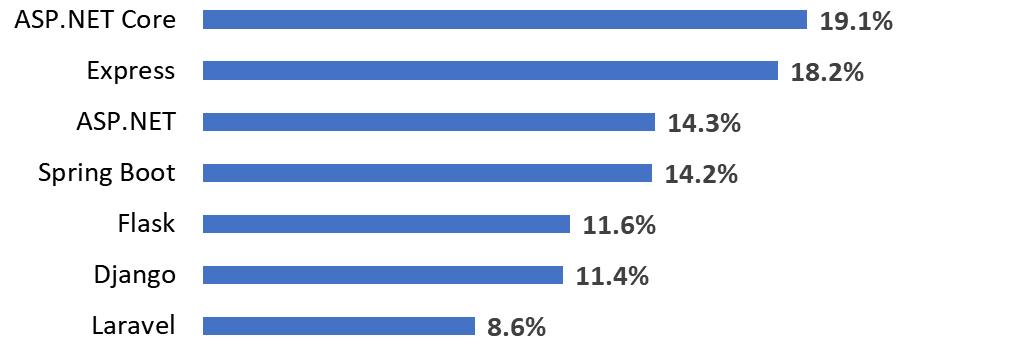
\includegraphics[width=0.9\linewidth]{images/Backend_Frameworks_Popularity.png}
  \caption{\label{Figure:Backend_Frameworks_Popularity}Web \ac{API} frameworks used by professional developers, adapted from~\cite{StackOverflow}}
\end{figure}
\FloatBarrier

The web \ac{API} frameworks present in Figure \ref{Figure:Backend_Frameworks_Popularity} are the following:
\begin{description}
  \item [ASP.NET Core/ASP.NET] ASP.NET Core is a high-performance and feature-rich framework developed by Microsoft. It is the successor to ASP.NET. Compared to its predecessor, ASP.NET Core offers many additional features and capabilities like increased performance, cross-platform compatibility, and native support for client-side development~\cite{Microsoft, Blinowski2022}. This framework uses the C\# programming language, demonstrating faster request processing compared to Django, Laravel, and frameworks based on Node.js.~\cite{ Haque2022, Madurapperuma2022, Blinowski2022}. ASP.NET Core is suitable for computationally-intensive or enterprise-scale applications due to its high performance and scalability~\cite{Ciliberti2017}.
  \item [Express] A flexible and minimalist framework that uses the Node.js environment, allowing server-side JavaScript execution, which explains its high popularity~\cite{Karlsson2021}. Due to its event-driven single-threaded nature, it is more resource-efficient than Django and ASP.NET Core, for example~\cite{Haque2022, Karlsson2021}. However, it is slower in processing CPU-intensive requests compared to ASP.NET Core and Spring Boot~\cite{Haque2022, Karlsson2021, Choma2023}. It also lacks some features natively present in other frameworks~\cite{Mozilla}. Still, Express is particularly effective for I/O-intensive applications, like chat and streaming applications~\cite{Karlsson2021, Zanevych2024}.
  \item [Spring Boot] An opinionated and feature-rich Java-based framework focused on ease of development. It reduces the need for configuration and generic code by providing starter dependencies, auto-configuration, default components, and more. It also offers real-time health status monitoring, metric reports, and traffic tracking. Spring Boot is especially suited for large-scale enterprise applications that use microservices~\cite{Mozilla, Zanevych2024, Blinowski2022}.
  \item [Flask] A lightweight and minimalist Python microframework. It is quite flexible and facilitates quick development, requiring no specific tools or libraries. Its design supports projects that start small and can be extended easily and customized as needed. Consequently, Flask is best suited for building resource-efficient microservices and smaller applications that require a high level of control.~\cite{Mozilla, Zanevych2024}.
  \item [Django] A scalable and feature-rich Python framework. It has a comprehensive list of features, including an \ac{ORM} tool that simplifies database operations, and an automatically generated administrator interface~\cite{Mozilla, Zanevych2024, Chen2017}. One of its drawbacks is slower request processing compared to other frameworks like ASP.NET Core and Spring Boot~\cite{Haque2022, Choma2023}. Despite that, it is suitable for both small-scale and large-scale applications~\cite{Mozilla, Zanevych2024}.
  \item [Laravel] A feature-rich framework built on the PHP programming language. Its toolset includes an \ac{ORM} database tool, versatile database migrations, and built-in task queuing and scheduling. This framework prioritizes concise and well-organized code. Laravel is suitable for both small projects and large-scale applications~\cite{Mozilla, Madurapperuma2022, Nguyen2022}.
\end{description}

\section{Monolithic \textit{vs.} Microservices Architecture}
\label{Section:Monolithic_vs_Microservices_Architecture}

The architectural design of a web \ac{API} is a decision that significantly impacts its development, deployment, scalability, and maintenance. When developing web \acp{API}, two dominant patterns emerge: the traditional monolithic approach and the modern microservices approach. Several papers highlight their benefits and drawbacks~\cite{Huf2019, Taibi2018, Adrio2023, Moysiadis2022}.

\subsection{Monolithic Architecture}
\label{Subsection:Monolithic_Architecture}

A monolithic architecture is a traditional model for software development in which the entire or most of the application is built as a single, tightly coupled unit. For a web \ac{API}, this means that all endpoints and their underlying logic are present within a single codebase and deployed as one unit~\cite{Taibi2018, Adrio2023, Moysiadis2022, Figueira2024, Kenan2020, Yoo2025}.

The main advantages of this approach are due to its basic nature. It offers simplicity of development, especially at the beginning of a project, because there is no burden from managing a distributed system. This centralized structure can also lead to improved performance, since calls between different components are direct function calls rather than network requests. A monolith is also easier to test, as requests tend to undergo fewer jumps between software components~\cite{Taibi2018, Adrio2023, Moysiadis2022, Figueira2024, Kenan2020, Blinowski2022}.

However, the monolithic model can be resource-inefficient since it is impossible to scale individual components independently. This architecture also imposes one particular technological framework on the entire application, reducing flexibility. In addition, because even a small change or issue can require the entire application to be recompiled and redeployed, it lowers resilience and deployment speed. All these issues only worsen as the application grows, leading to decreased scalability and maintainability, as well as possibly negating some of its advantages~\cite{Taibi2018, Adrio2023, Moysiadis2022, Figueira2024, Kenan2020, Villamizar2015}.

\FloatBarrier
\begin{figure}[H]
  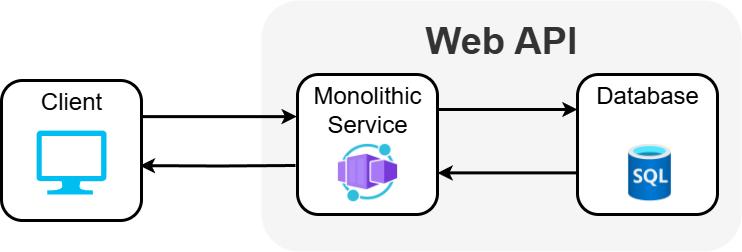
\includegraphics[width=0.9\linewidth]{images/MonolithicArchitecture.png}
  \caption{\label{Figure:Monolithic_Architecture}Example of a Monolithic Architecture}
\end{figure}
\FloatBarrier

\subsection{Microservices Architecture}
\label{Subsection:Microservices_Architecture}

A microservices architecture follows a \ac{SOA}, structuring an application as a collection of small and loosely coupled services. Each service is self-contained, responsible for a specific business goal, and may communicate with other services~\cite{Taibi2018, Adrio2023, Moysiadis2022, Khalfaoui2025, Figueira2024, Kenan2020}.

The microservices architecture offers superior scalability, as each service can be scaled independently based on its specific load, which is a highly efficient model for cloud-based deployments. This decoupling also allows a heterogeneous technology stack, for example, one service may use the ASP.NET Core framework while another uses the Spring Boot framework. Furthermore, this type of architecture is more resilient, as the failure of a single service does not necessarily compromise the entire application. Additionally, this architecture improves maintainability by breaking a large application down into smaller and more understandable codebases. Developers can work on individual services, allowing them to develop, deploy, and update their components autonomously~\cite{Taibi2018, Adrio2023, Moysiadis2022, Khalfaoui2025, Figueira2024, Kenan2020, Villamizar2015}.

However, the microservices pattern introduces some challenges. One drawback is the increased implementation effort, since developers must implement mechanisms for inter-service communication. This leads directly to communication and network complexity. Instead of simple function calls, services must communicate over a network, introducing considerations of latency, security, and fault tolerance~\cite{Taibi2018, Adrio2023, Khalfaoui2025, Figueira2024, Kenan2020, Villamizar2015, Yoo2025}.

To address some challenges inherent to the microservice architecture, the API Gateway pattern is often recommended. In this pattern, an API Gateway acts as an intermediary for all client requests, simplifying the client-side logic. Instead of clients needing to know the addresses of and communicate with multiple services, they make requests to the gateway only. The gateway then routes requests to the appropriate microservice, and can also aggregate responses from multiple services into a single response. It may handle concerns such as authentication and rate limiting as well~\cite{Taibi2018, Adrio2023, Khalfaoui2025, Kenan2020}.

Regarding data management, multiple approaches may be applied when dealing with microservices, ranging from a single shared database for all services, to one database per service. Sharing a single database is simpler and facilitates data integrity, but is less scalable and flexible. In contrast, using one database per service offers greater scalability and flexibility, but increases complexity and adds the challenge of maintaining data integrity between services~\cite{Taibi2018, Khalfaoui2025, Kenan2020}.

Figure \ref{Figure:Microservices_Architecture} shows an example of a microservice architecture adhering to the \ac{API} Gateway and database-per-service patterns.

\FloatBarrier
\begin{figure}[H]
  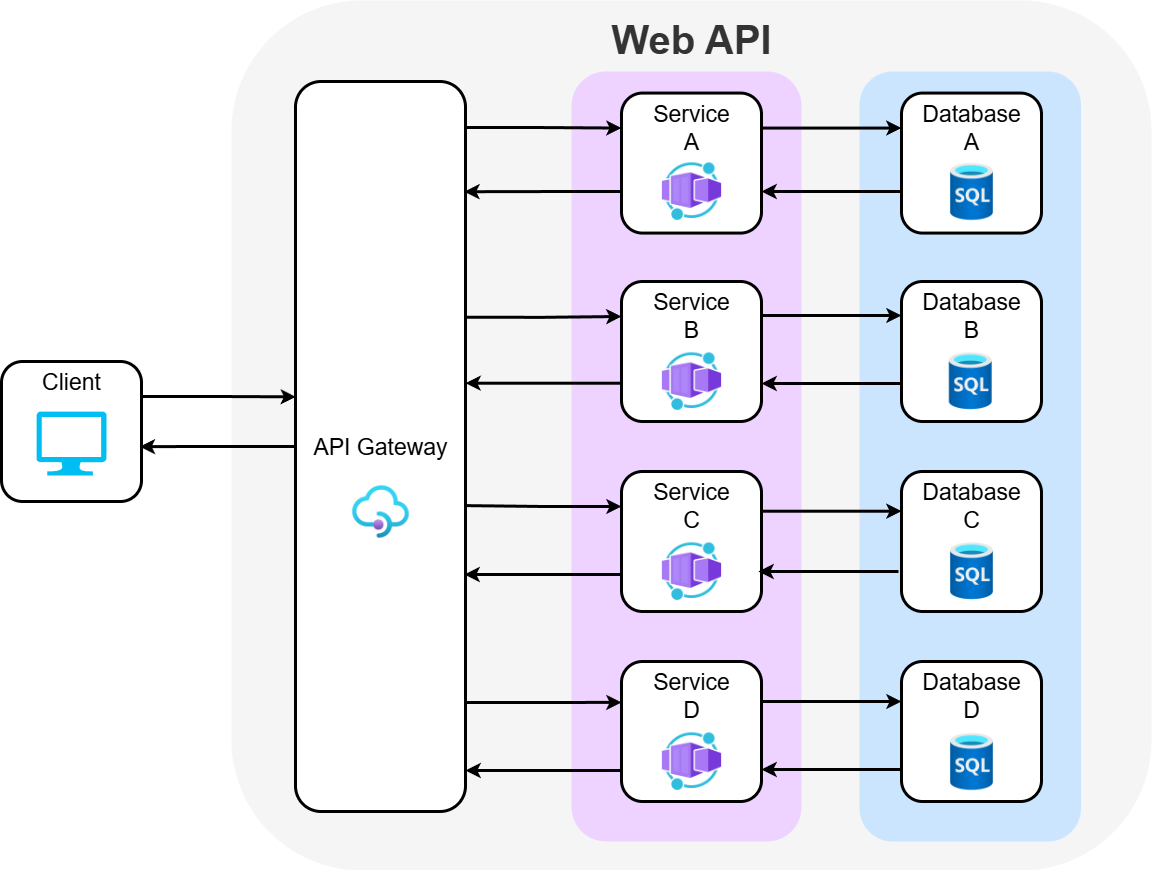
\includegraphics[width=0.9\linewidth]{images/MicroservicesArchitecture.png}
  \caption{\label{Figure:Microservices_Architecture}Example of a Microservices Architecture}
\end{figure}
\FloatBarrier

\section{Cloud Computing}
\label{Section:Cloud_Computing}

Cloud computing is the provision of on-demand \ac{IT} services to customers over the Internet. These services may consist of software applications, databases, analytics, servers, and more. The resources are hosted on a remote server (the "cloud") located in a provider's data center, and accessible through a web browser~\cite{Figueira2024,  Nordic2012, Nadeem2024, Villamizar2016}.

Cloud services can be divided into three distinct models:
\begin{description}
  \item [\ac{IaaS}] Provides processing power, storage, and network capabilities through a \ac{VM}. The customer is responsible for the \ac{OS}, runtimes, applications, and data. This model is quite flexible and is suitable for companies that want to improve the reliability and scalability of their infrastructure~\cite{Figueira2024, Nordic2012, Google, Berry2021}.
  \item [\ac{PaaS}] Offers an environment to build, deploy, and run applications without managing the associated hardware and software components. The customer can focus on developing applications and handling data, making this model is useful for software engineers and developers~\cite{Figueira2024, Nordic2012, Google, Berry2021}.
  \item [\ac{SaaS}] Provides a ready-to-use application fully managed by the cloud provider. This model is designed for end users of the application and organizations that wish to offer it to their employees~\cite{Figueira2024, Nordic2012, Google, Berry2021}.
\end{description}

Figure \ref{Figure:CloudServiceModels} illustrates the differences between these three service models and the self-hosting approach, where the customer is responsible for all components.

\FloatBarrier
\begin{figure}[H]
  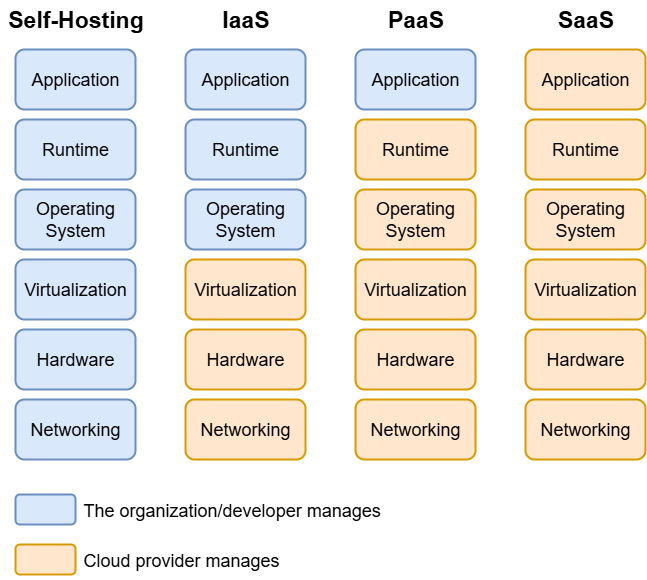
\includegraphics[width=0.7\linewidth]{images/CloudServiceModels.png}
  \caption{\label{Figure:CloudServiceModels}Cloud service models}
\end{figure}
\FloatBarrier

Cloud computing has several advantages over self-hosting. It prevents expensive asset acquisitions and reduces maintenance costs because resources are only paid for when they are actually needed. Furthermore, it allows companies to scale their services as required, since cloud resources can be purchased in practically any quantity and readjusted fast. Cloud providers also have fallback data centers they can resort to in case of failure without affecting the user experience, improving reliability. Finally, by providing on-demand infrastructure, cloud computing speeds up the development and testing of new solutions while decreasing financial risk, promoting innovation~\cite{Figueira2024, Nordic2012, Alam2020, Nadeem2024, Villamizar2016}.

Nevertheless, cloud computing also has some disadvantages. Choosing a cloud-based service means that a third-party organization, possibly a foreign one, now manages sensitive data. This raises security issues, as well as legal considerations related to data protection regulations. Another drawback is low interoperability; once a company chooses a particular cloud provider, changing to another or working with multiple is difficult. In addition, the limited flexibility and customization of cloud computing can inhibit integration with certain systems~\cite{Nordic2012, Alam2020}.

Overall, cloud computing is changing the way businesses deliver their software solutions. It is democratizing the impact of \ac{IT} by giving companies of any size instant access to high-quality computing infrastructure. With this technology, software developers can develop and deploy web applications faster while reducing costs~\cite{Figueira2024, Berry2021, Nadeem2024}.

\section{Containerization}

Containerization is an approach to deploying software where an application, along with all its necessary dependencies (libraries, frameworks, configuration files, etc.), is packaged into a single unit called a container. Containerization is a virtualization technology that is popular in cloud and microservice environments due to its beneficial characteristics~\cite{Figueira2024, Hardikar2021, Potdar2020}.

Containers are portable and self-sufficient packages, which ensures they run consistently across different environments. This consistency reduces deployment issues and makes it easier to set up new environments. Additionally, unlike regular \acp{VM}, containers virtualize their \ac{OS}, meaning they only contain the application itself, with no \ac{OS} overhead. Because of this, containers use less memory and \ac{CPU} power, making them more efficient and scalable than \acp{VM}~\cite{Figueira2024, Hardikar2021, Potdar2020}.

Docker is the leading container platform. It automates and standardizes the deployment of applications inside software containers by providing an additional layer of abstraction to the containerization process. To create a container, Docker uses a Dockerfile, a text-based script of instructions used to create a container image. This immutable image is a lightweight, standalone, executable package that contains everything needed to run an application. When the image is run, it becomes a container, which is an active instance of the image~\cite{Figueira2024, Hardikar2021, Potdar2020}.

\section{Literature Review Conclusion}
\label{Section:Literature_Review_Conclusion}

The literature review presented in this chapter highlighted the main concepts and technologies relevant to this dissertation.

First, an overview of freight transportation, the business domain of the web \ac{API} to be developed, was provided. This overview was useful to understand the commercial purpose of the web \ac{API} and its functional requirements.

Then, this literature review covered the concept of web \acp{API}, their specifications, security methods, and popular development frameworks. In the context of this dissertation, web \acp{API} represent the server-side of web applications. Web \acp{API} expose an interface that allows clients to interact with the server's resources. The most popular specifications for web \acp{API} are \ac{REST}, GraphQL, and \ac{RPC}. Regarding security, authentication and authorization mechanisms like \ac{OAuth} 2.0, \ac{OIDC}, and \ac{JWT} are essential to protect sensitive operations and data. The source code a web \ac{API} can be simplified and standardized by using a framework intended for this type of software.

After that, two architectural patterns for web \acp{API} were discussed, explaining the advantages and disadvantages of a microservices architecture compared to a monolithic one. The microservice-based architecture has many benefits, especially in large-scale applications, but it also introduces complexity.

Finally, cloud computing and containerization were presented. Cloud computing allows companies to access high-quality infrastructure and services on demand, simplifying the deployment and management of web applications. Containerization is a virtualization technology that improves the portability, consistency, and efficiency of deployed applications.

One key characteristic of this literature review is the lack of studies that contribute with a comprehensive architectural approach for web \acp{API} or web applications. The few documents that do exist tend to focus on specific aspects of web \ac{API} architecture, such as security or scalability, rather than providing a holistic view. Chapters \ref{Chapter:Design_And_Architecture} and \ref{Chapter:Implementation} intend to address this issue by detailing the design, architecture, and implementation of a web \ac{API} that follows modern practices described in this literature review.

\chapter{Design and Architecture}
\label{Chapter:Design_And_Architecture}

This chapter details the design and architecture of the web \ac{API} developed in this dissertation. This process was driven by the theoretical knowledge presented in Chapter \ref{Chapter:Literature_Review} and the specific software requirements listed in Section \ref{Section:Requirements}.

\section{Requirements}
\label{Section:Requirements}

The design and architecture of the web \ac{API} are guided by a specific list of software requirements. These include functional requirements that establish the system's features, and non-functional requirements that determine the attributes of the system and how it should operate. Every requirement is listed below:

\begin{requirement}
  \label{Requirement:1}
  Provide freight quotes to users by querying external carrier \acp{API} (WebCargo for air, Cargofive for sea) for freight rates. To achieve this, the system must expose an endpoint that accepts a payload containing the origin, destination, and other parameters, depending on the transport mode.
\end{requirement}

\begin{requirement}
  \label{Requirement:2}
  Provide users with their quote search history via a GET request, which contains both the requests they made and the responses they received from the web \ac{API}. The results must support pagination.
\end{requirement}

\begin{requirement}
  \label{Requirement:3}
  Allow only users with the administrator role to access information about any user of the web \ac{API}.
\end{requirement}

\begin{requirement}
  \label{Requirement:4}
  Expose endpoints for querying supported airports and seaports. The query must have pagination and search term options.
\end{requirement}

\begin{requirement}
  \label{Requirement:5}
  When a user deletes their account, also delete all associated data from the databases.
\end{requirement}

\begin{requirement}
  \label{Requirement:6}
  Restrict the functionalities described in Requirements \ref{Requirement:1}, \ref{Requirement:2}, and \ref{Requirement:3} to authenticated users only.
\end{requirement}

\begin{requirement}
  \label{Requirement:7}
  In case of a complete failure in one external carrier \ac{API} integration, the rest of the system must remain operational.
\end{requirement}

\begin{requirement}
  \label{Requirement:8}
  Support decoupled and automatic scaling of the web \acp{API}'s request processing capabilities based on real-time use of specific endpoints.
\end{requirement}

\begin{requirement}
  \label{Requirement:9}
  Freight rates from external carrier \acp{API} must be cached for 1 day to avoid reaching rate limits.
\end{requirement}

\begin{requirement}
  \label{Requirement:10}
  When serving concurrent 200 users sending basic GET requests, the 90th percentile response time must be less than 500 milliseconds. Basic GET requests are those that simply retrieve a database record based on its unique identifier from the database.
\end{requirement}

\begin{requirement}
  \label{Requirement:11}
  Enforce a single public entry point to access the web \ac{API}'s resources.
\end{requirement}

\begin{requirement}
  \label{Requirement:12}
  Authentication must be done securely via the \ac{OAuth} 2.0 and \ac{OIDC} protocols, without storing user credentials in the system's databases.
\end{requirement}


Requirements \ref{Requirement:1} to \ref{Requirement:5} are functional, whereas Requirements \ref{Requirement:6} to \ref{Requirement:12} are non-functional. Requirement \ref{Requirement:1} was explicitly specified by the industry partner Devlop, representing the web \ac{API}'s main functionality. To expand its scope, others were added as reasonable requirements for a real-world, enterprise web \ac{API}.

\section{High-Level Architecture}
\label{Section:High_Level_Architecture}

The high-level architecture focuses on the main components of the system and concisely describes their roles. For the remainder of this document, the names of all major components will be capitalized. Figure \ref{Figure:High_Level_Architecture} shows the high-level architecture of the web \ac{API}.

\begin{figure}[H]
  \centering
  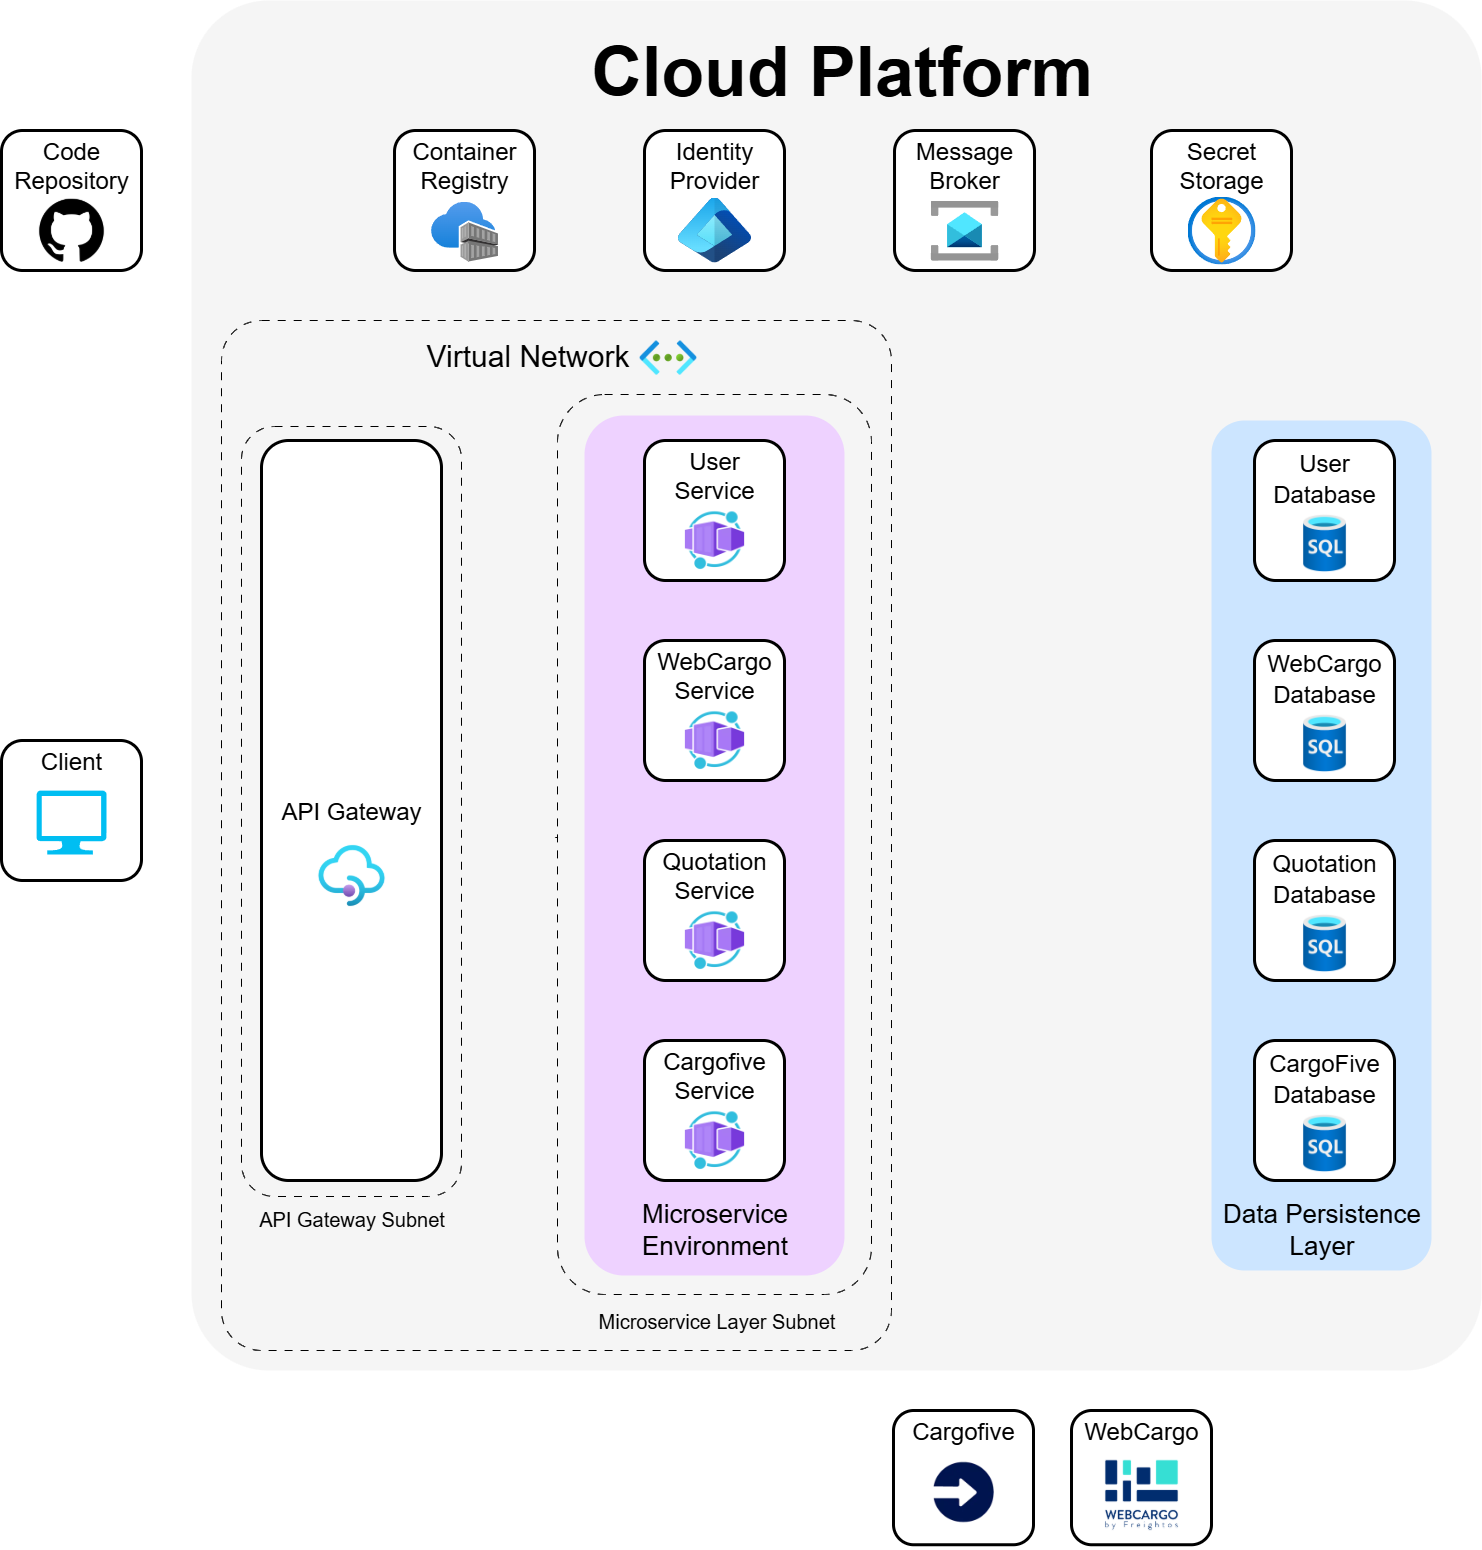
\includegraphics[width=1\linewidth]{images/HighLevelArchitecture.png}
  \caption{\label{Figure:High_Level_Architecture}High-Level Architecture}
\end{figure}

\subsection{Client}

The Client is the user-facing application that serves as the primary interface to the system. It is a decoupled frontend from another project, implemented as a \ac{SPA}. Its main responsibilities are to render the \ac{UI}, manage user sessions, and communicate with the \ac{API} Gateway for data and functionality. For user authentication and account management, the Client directs users to a dedicated page on the Identity Provider, where they can log in, log out, delete their account, etc.

\subsection{\texorpdfstring{\ac{API}}{API} Gateway}
\label{Subsection:API_Gateway}

The \ac{API} Gateway functions as the single entry point for all incoming Client requests, similarly to the pattern described in Subsection \ref{Subsection:Microservices_Architecture}. This component routes requests to the appropriate microservice, allowing the Client to interact with the system without needing to know what microservices it contains. The \ac{API} Gateway also enforces authentication by validating access tokens (\acp{JWT}).

\subsection{Microservice Environment}
\label{Subsection:Microservice_Environment}

The Microservice Environment holds the core of the system's business logic, implemented following a microservices architectural style described in Subsection \ref{Subsection:Microservices_Architecture}. The microservices in this environment are designed around specific business goals, communicating with each other directly through endpoints exposed between them, or indirectly through the Message Broker component. In this web \ac{API}, each microservice enforces its own authorization policies, restricting access to resources based on roles or more complex business rules. In addition, every microservice runs in a Docker container.
There are four microservices in this environment, which are considered major components of the system:
\begin{description}
  \item[User Service] This service provides endpoints to retrieve user-related information. To do so, it communicates with the Identity Provider. It also communicates with the Identity Provider to be informed about user deletions, which it propagates to the rest of the system through the Message Broker. Even though User Service does not store user data, it still needs an associated database to store data related to the Identity Provider. The purpose of this data will be explained in Chapter \ref{Chapter:Implementation}.
  \item[Quotation Service] This service orchestrates the core freight quotation business logic. It communicates with WebCargo Service and Cargofive Service to obtain freight rates and uses them to calculate and store freight quotes based on user input received through the \ac{API} Gateway. Users can fill out a freight quote request and obtain a response with a freight quote, as well as retrieve their quote history. Quotation Service also stores data relevant to the general quotation process, including locations (airports and seaports), special handling codes, and cargo container types. This general data is anonymously accessible through endpoints.
  \item[WebCargo Service] This service is responsible for all business logic related to the WebCargo external \ac{API}, which is used to obtain up-to-date air freight rates. It extracts all relevant information present in the freight rates retrieved from the WebCargo \ac{API} and stores them in the corresponding database. Most importantly, it provides air freight rates to Quotation Service when requested.
  \item[Cargofive Service] Analogously to the WebCargo Service, this service interacts with the Cargofive external \ac{API} to fetch current sea freight rates. It extracts all relevant information present in the retrieved freight rates and stores them in its associated database. Its defining role is to supply freight rate data to Quotation Service upon request.
\end{description}

\subsection{\texorpdfstring{\ac{VNet}}{VNet}}

The \ac{VNet} provides network isolation for the system's components in the cloud platform. The Microservice Environment and the API Gateway reside in the \ac{VNet}, each in its dedicated subnet. The main objective of these dedicated subnets is to implement network segmentation, enforcing network policies that apply to all inbound and outbound traffic. Specifically, the \ac{API} Gateway subnet is configured to allow inbound traffic from the Internet, while the Microservice Environment subnet only accepts traffic from within the \ac{VNet}. Furthermore, components within the \ac{VNet} can securely access other components (the Message Broker, the Secret Storage, and the Data Persistence Layer) via private endpoints, which integrate them directly into the \ac{VNet}'s address space.

\subsection{Data Persistence Layer}

The Data Persistence Layer manages the persistent storage of the web \ac{API}'s data. This layer may consist of multiple database technologies, as each microservice owns its data and communicates with its corresponding database. Access to this layer is secured through a private endpoint within the VNet.

\subsection{Identity Provider}
\label{Subsection:Identity_Provider}

The Identity Provider is an external service responsible for all user authentication and account management. It implements the \ac{OAuth} 2.0 and \ac{OIDC} protocols to authenticate users and issue \acp{JWT} to the Client. By delegating authentication and account management to an instance of a specialized Identity Provider, the system avoids storing user credentials and benefits from enterprise-level security features, such as multifactor authentication.

\subsection{Message Broker}
\label{Subsection:Message_Broker}

The Message Broker facilitates asynchronous communication between microservices and employs a publish-subscribe model. This component is useful when one service must send a notification or delegate a task but does not need to know the exact recipients nor receive a direct response. The Message Broker also implements mechanisms for message durability and delivery guarantees in case a microservice subscribes to a topic after messages have already been published. In this web \ac{API}, the Message Broker is utilized when User Service needs to notify the system that a user has been deleted. In addition, it is used when Cargofive Service needs to synchronize data with Quotation Service. The Message Broker is accessed through a private endpoint within the VNet.

\subsection{Secret Storage}

The Secret Storage is a centralized and secure repository for all application secrets. This contains \ac{API} keys for external carrier \acp{API} (WebCargo and Cargofive) and the secret value to access the Identity Provider instance as an administrator. The microservices access the Secret Storage at runtime by a private endpoint within the VNet.

\subsection{WebCargo and Cargofive \texorpdfstring{\acp{API}}{APIs}}

The WebCargo and Cargofive \acp{API} are third-party dependencies that provide essential business functionality not built in the system. The system integrates with these \acp{API} to retrieve up-to-date freight rates from many carriers, as explained in Subsection \ref{Subsection:Microservice_Environment}. WebCargo Service and Cargofive Service communicate with the WebCargo and Cargofive \acp{API} respectively, using the \ac{API} keys supplied by Devlop for authentication. Each of these external \acp{API} has its own documentation and usage policies. Furthermore, the WebCargo \ac{API} returns responses in \ac{XML} format, while the Cargofive \ac{API} uses \ac{JSON}.

\subsection{Code Repository}

The Code Repository is the version control system that stores the source code of all microservices and \ac{CI/CD} pipeline workflows. These workflows automate the build and deployment process and are triggered when the source code is updated. These workflows access the Container Registry and the Microservice Environment components through privately stored secrets.

\subsection{Container Registry}

The Container Registry is a private repository for storing and managing the versioned container images for each microservice. During the \ac{CI/CD} process, new Docker images are built and pushed to the registry. Subsequently, these images are pulled from the registry to be run as Docker containers, where each container is an instance of a particular microservice within the Microservice Environment.

\section{Runtime Communication}
\label{Section:Runtime_Communication}

The architecture presented in Section \ref{Section:High_Level_Architecture} defines a set of components. These components must communicate with each other to achieve their objectives. This Section explains the web \ac{API}'s runtime communication, which refers to the exchange of data between components that typically occurs while the microservices are running.

\subsection{Client-Server Communication}
\label{Subsection:Client_Server_Communication}

The client-server communication includes all requests sent by the Client to a server-side component: either the \ac{API} Gateway or the Identity Provider. It also includes the \ac{API} Gateway routing to the correct microservice, since successful Client requests are ultimately handled in the Microservice Environment. Figure \ref{Figure:ClientServerCommunication} illustrates these interactions.

\begin{figure}[H]
  \centering
  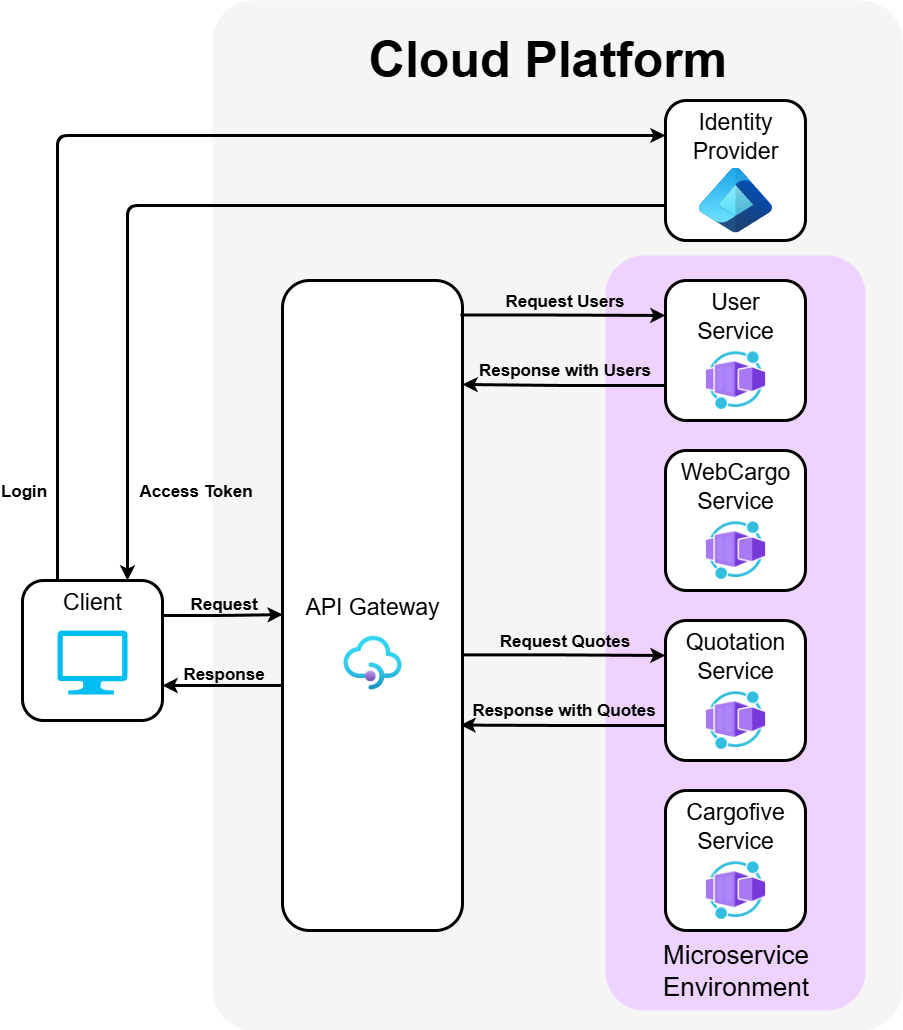
\includegraphics[width=0.9\linewidth]{images/ClientServerCommunication.png}
  \caption{\label{Figure:ClientServerCommunication}Client-Server Communication}
\end{figure}

The Client initiates authentication by redirecting users to the Identity Provider's login page. After a successful login, the Identity Provider redirects the user back to the Client with an authorization code. The Client then exchanges this code for an access token (\ac{JWT}) by making a request to the Identity Provider's token endpoint, completing the authentication process.

The Client sends requests to the \ac{API} Gateway to access the web \ac{API}'s resources. If the particular resource requires authentication, the \ac{API} Gateway first validates the access token included in the request's authorization header. Then, if the token is valid or no authentication is needed, the \ac{API} Gateway routes the request to the appropriate microservice in the Microservice Environment. The microservice processes the request and sends a response back to the \ac{API} Gateway, which forwards it to the Client.

\subsection{Identity Provider Communication}

User Service exposes endpoints that allow the Client to get information about users. Since the Identity Provider is responsible for storing user accounts, User Service communicates with it to retrieve user data. This communication is shown in Figure \ref{Figure:IdentityProviderCommunication}. Additionally, User Service subscribes to user account deletion notifications from the Identity Provider.

\begin{figure}[H]
  \centering
  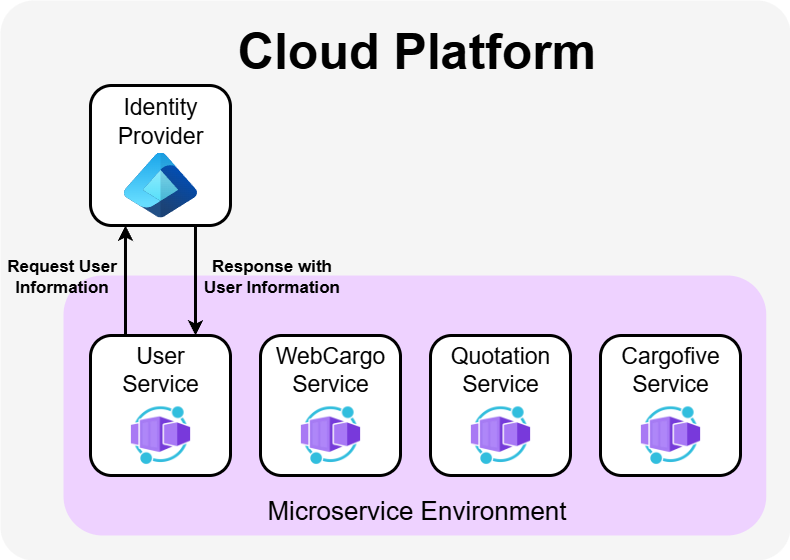
\includegraphics[width=0.9\linewidth]{images/IdentityProviderCommunication.png}
  \caption{\label{Figure:IdentityProviderCommunication}Identity Provider Communication}
\end{figure}

\subsection{Database Communication}

Each microservice establishes a connection to its correspondent database and performs the necessary queries to retrieve or modify data. Access to the Data Persistence Layer is secured through a private endpoint within the VNet. Figure \ref{Figure:DatabaseCommunication} illustrates the communication between microservices and their databases.

\begin{figure}[H]
  \centering
  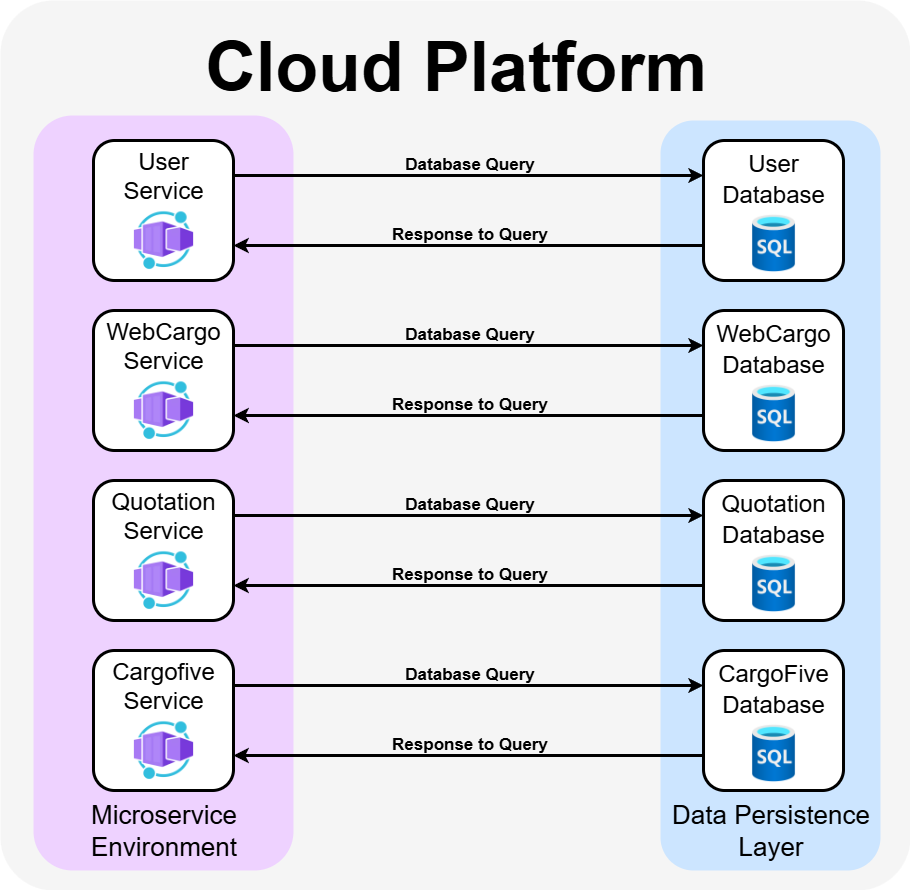
\includegraphics[width=0.9\linewidth]{images/DatabaseCommunication.png}
  \caption{\label{Figure:DatabaseCommunication}Database Communication}
\end{figure}

\subsection{Direct Inter-Service Communication}
\label{Subsection:Direct_Inter_Service_Communication}

Microservices can communicate with each other directly by making \ac{HTTP} requests to each other's endpoints. Some of these endpoints may only be reachable to other services, not the Client. This allows for real-time data exchange and coordination between services.

The web \ac{API} makes use of this type of communication when Quotation Service needs to obtain freight rates from WebCargo Service or Cargofive Service, as shown in Figure \ref{Figure:DirectCommunication}.

\begin{figure}[H]
  \centering
  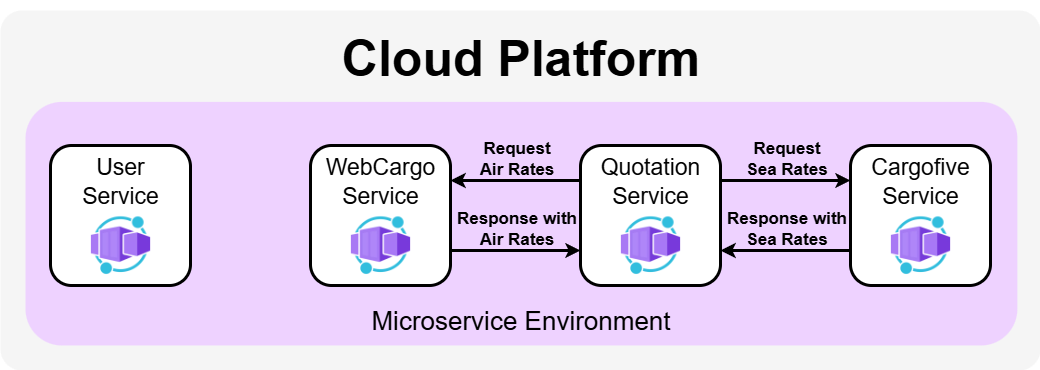
\includegraphics[width=1\linewidth]{images/DirectCommunication.png}
  \caption{\label{Figure:DirectCommunication}Direct Inter-Service Communication}
\end{figure}

\subsection{Event-Driven Inter-Service Communication}
\label{Subsection:Event_Driven_Inter_Service_Communication}

Event-driven communication is applied in two scenarios using the Message Broker, as explained in Subsection \ref{Subsection:Message_Broker}.

The first scenario occurs when a user deletes their account through the Identity Provider.

Firstly, User Service must be informed about the deletion to propagate it to the rest of the system. To achieve this, it can either poll the Identity Provider periodically or subscribe to its user deletion notifications. Once User Service is informed, it publishes a "UserDeleted" event to the Message Broker containing the identifier of the deleted user. Finally, Quotation Service receives this event and deletes the quotation search history of the deleted user from its database. The user deletion event process is shown in Figure \ref{Figure:EventDrivenCommunicationUserDeleted}.

\begin{figure}[H]
  \centering
  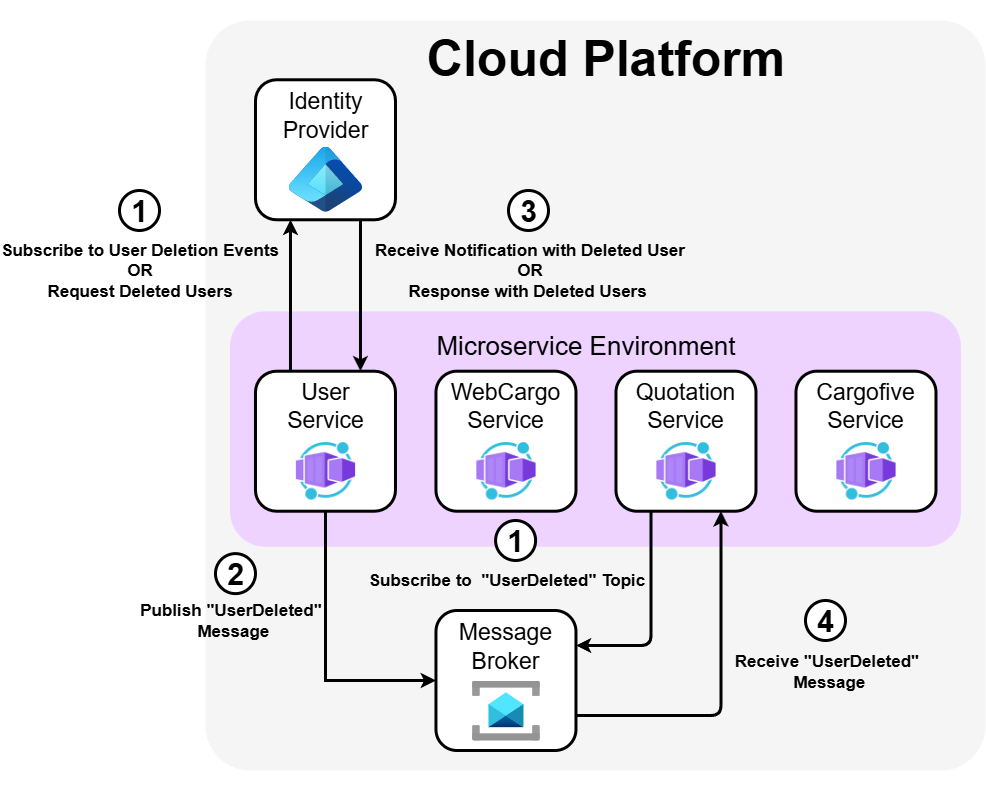
\includegraphics[width=0.9\linewidth]{images/EventDrivenCommunicationUserDeleted.png}
  \caption{\label{Figure:EventDrivenCommunicationUserDeleted}Event-Driven Inter-Service Communication: User Deleted}
\end{figure}

The second scenario occurs when Cargofive Service needs to synchronize data with Quotation Service. This synchronization is necessary because the Cargofive \Ac{API} uses its own identifiers for seaports, unlike the WebCargo \ac{API}, which can identify airports through standardized codes. Cargofive Service fetches the list of supported seaports from the Cargofive \ac{API} weekly. Cargofive Service publishes a "SeaportsUpdated" event to the Message Broker containing the relevant data. Quotation Service is subscribed to this event, so it is notified and updates its database if necessary. This process is shown in Figure \ref{Figure:EventDrivenCommunicationCargofive}.

\begin{figure}[H]
  \centering
  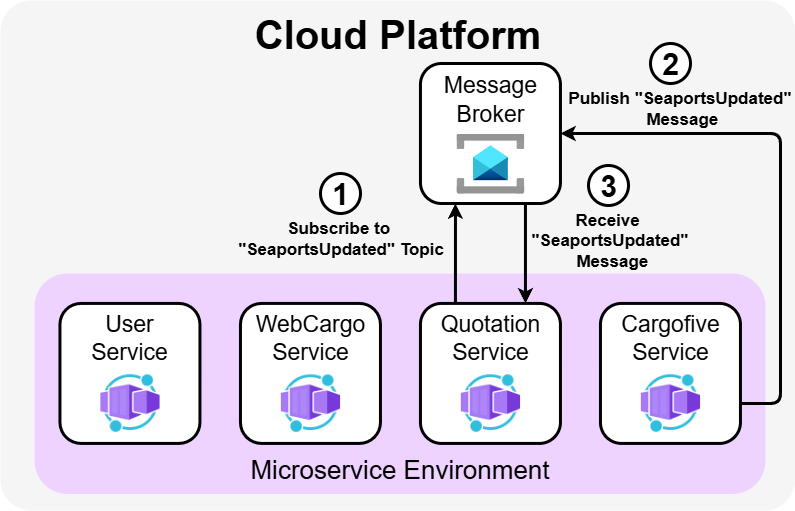
\includegraphics[width=0.9\linewidth]{images/EventDrivenCommunicationCargofive.png}
  \caption{\label{Figure:EventDrivenCommunicationCargofive}Event-Driven Inter-Service Communication: Cargofive Synchronization}
\end{figure}

\subsection{External Carrier API Communication}
\label{Subsection:External_Carrier_API_Communication}

WebCargo Service and Cargofive Service communicate with the WebCargo and Cargofive \acp{API}, respectively. The two services use the \acp{API} as clients to send requests and receive responses, as shown in Figure \ref{Figure:ExternalCarrierAPICommunication}. The \ac{API} keys required for authentication are retrieved from the Secret Storage at runtime and stored in memory.

\begin{figure}[H]
  \centering
  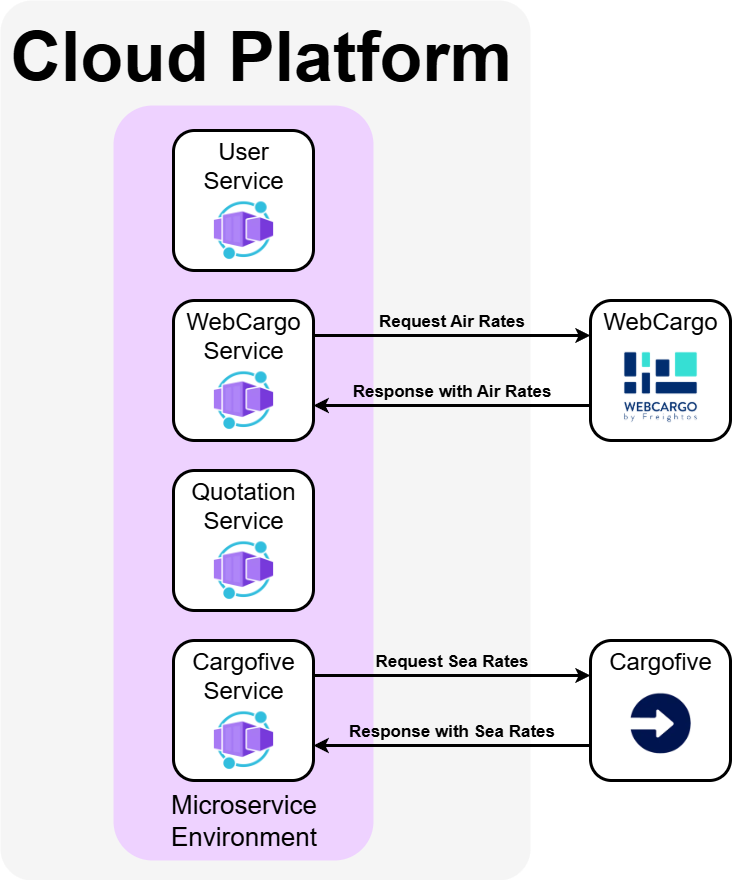
\includegraphics[width=0.9\linewidth]{images/ExternalCarrierAPICommunication.png}
  \caption{\label{Figure:ExternalCarrierAPICommunication}External Carrier \ac{API} Communication}
\end{figure}

\section{\texorpdfstring{\ac{API}}{API} Specification}
\label{Section:API_Specification}

The \ac{API} specification is a document that lays out the endpoints, data schemas, and request-response formats of the web \ac{API}, providing a clear notion of how to interact with it. Figure \ref{Figure:API_Specification} shows the web \ac{API}'s specification, which adheres to the OpenAPI standard\footnote{OpenAPI Specification, \url{https://swagger.io/specification/}, (accessed 31 Aug. 2025)}. This document contains all endpoints that the microservices expose to the Client through the \ac{API} Gateway.

\begin{figure}[H]
  \centering
  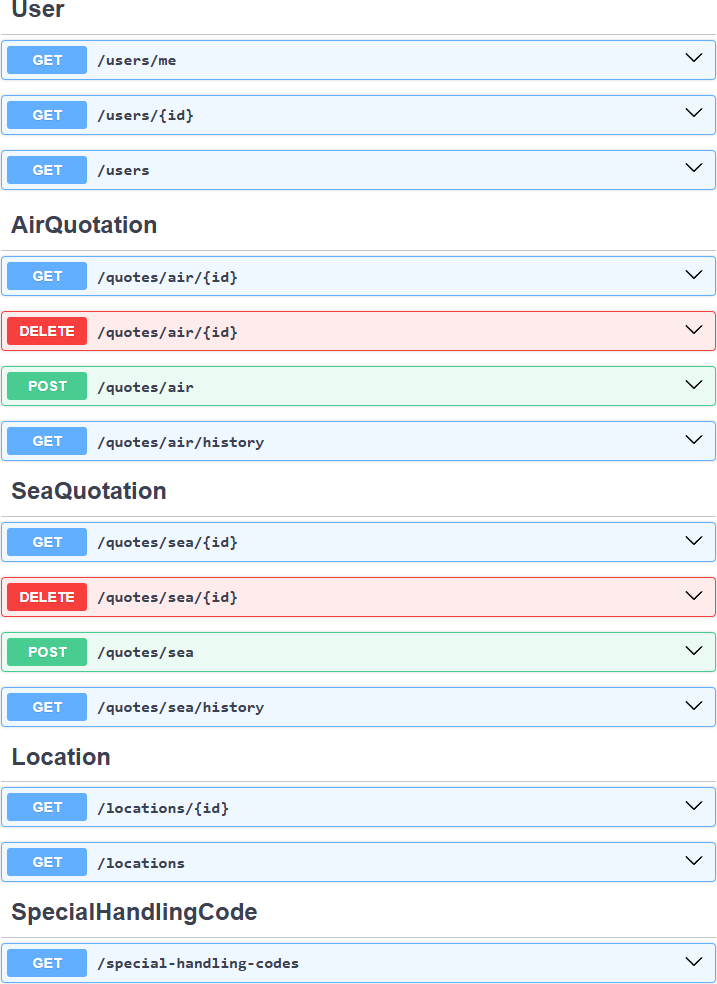
\includegraphics[width=0.85\linewidth]{images/API_Specification.png}
  \caption{\label{Figure:API_Specification}\ac{API} Specification}
\end{figure}

\section{Internal Architecture of the Microservices}
\label{Section:Internal_Architecture_Microservices}

In the web \ac{API}, the source code of each microservice adheres to a similar architecture. Figure \ref{Figure:InternalMicroserviceArchitecture} shows the main modules of this architecture and their interactions, where all arrows inside the "Microservice" region represent function calls in the running program. Each module is designed to handle specific types of tasks and responsibilities, promoting code modularity and maintainability. The next subsections explain the purpose of each module.

\begin{figure}[H]
  \centering
  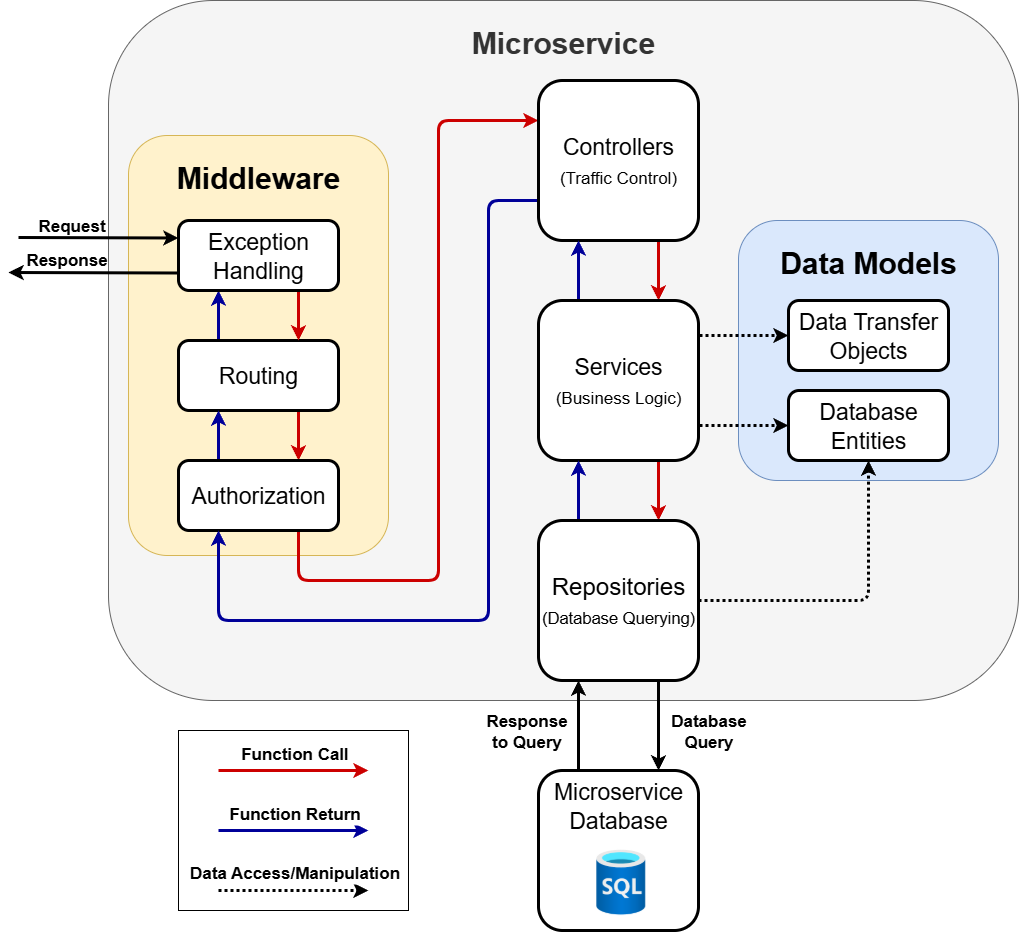
\includegraphics[width=1\linewidth]{images/InternalMicroserviceArchitecture.png}
  \caption{\label{Figure:InternalMicroserviceArchitecture}Internal Architecture of a Microservice}
\end{figure}

\subsection{Middleware}
\label{Subsection:Middleware}

The middleware pipeline directly interacts with incoming requests and outgoing responses in a specified order of middleware processes. Each process can inspect or change the request or response. In the web \ac{API} being designed, three middleware processes are applied in this exact order:

\begin{description}
  \item[Exception Handling] This process is invoked at the beginning of the request pipeline. If an unhandled error occurs during the processing of a request, it catches the error and generates a response with a fitting error code and message.
  \item[Routing] This process is responsible for matching incoming requests to the appropriate endpoint based on the request's specified destination. The destination of the request depends on its \Ac{URL} and \ac{HTTP} method.
  \item[Authorization] This process checks whether the authenticated user has the necessary permissions to access the requested resource. If the user lacks the required permissions, it blocks the request and generates a response with a "403 Forbidden" status code. For endpoints that allow anonymous access, this process has no effect. Authentication and authorization requirements are defined in the controller modules.
\end{description}

\subsection{Data Models}

Data models represent business data structures. In the web \ac{API}'s source code, they correspond to objects that are designed for data encapsulation but contain no business logic. There are two types of data models:

\begin{description}
  \item[\acp{DTO}] These objects hold business data and may contain validation or transformation logic. Microservice components use \acp{DTO} for data interchange in many \ac{API} interactions, including those with the Client, other microservices, and the external carrier \acp{API}.
  \item[Database Entities] These data models represent database tables and are used to map the microservice's business data to the the correspondent database schema. An instance of an entity is equivalent to a row in the database table it represents. Entities allow the database schema to be programmatically defined in the microservice's source code.
\end{description}

\subsection{Controllers}

Controllers are responsible for handling requests routed by the middleware. Each controller defines one or more endpoints corresponding to a specific resource (location, user, freight quote, etc.) or functionality of the microservice. These modules control traffic by specifying each endpoint's authentication and authorization requirements, as well as their expected input and output parameters. Controllers interact with the necessary Service modules to fulfill the request and initiate a response with relevant data to the Client.

\subsection{Services}

Service modules execute the core business logic of the microservice and coordinate interactions between other modules. They use \acp{DTO} to exchange data with external \acp{API}, the Client, and other microservices. These modules can create database entity instances directly to then store them in the database by interacting with repository modules. Service modules also interact with repository modules to retrieve, modify, or delete database records.

\subsection{Repositories}

Repositories provide functions for database access and manipulation. They act as an abstraction layer between the service modules and the database, holding the logic required to interact with the microservice's database. Repositories use database entity instances to perform \ac{CRUD} operations on behalf of service modules. Furthermore, repository modules are agnostic to specific database technologies.

\section{Deployment}
\label{Section:Deployment}

The web \ac{API}'s microservices are deployed to the cloud platform through a \ac{CI/CD} pipeline. This pipeline automates the build, test, and deployment processes, ensuring that the relevant microservice instances running in the cloud are promptly updated. The \ac{CI/CD} pipeline is triggered whenever a change is pushed to the master branch of the Code Repository. Figure \ref{Figure:Deployment} illustrates the two main steps of the deployment process.

\begin{figure}[H]
  \centering
  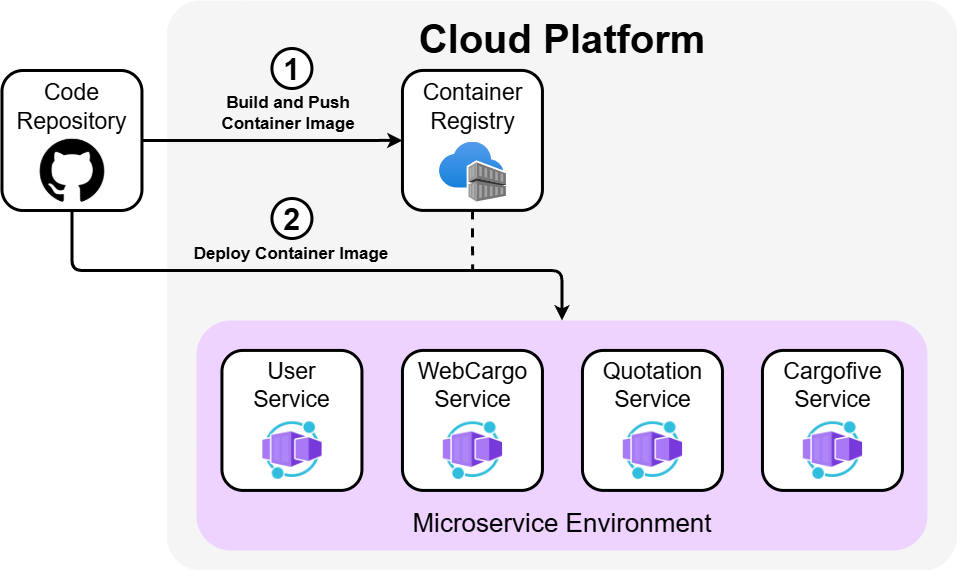
\includegraphics[width=0.9\linewidth]{images/Deployment.png}
  \caption{\label{Figure:Deployment}Deployment to the Cloud Platform}
\end{figure}

In the first stage, the source code is compiled with a production-ready configuration and built into a container image, which is then pushed to the Container Registry. In the second stage, the container image is deployed to the cloud platform's container orchestration service (the Microservice Environment), where it is run in a scalable and supervised environment. Both of these stages involve authenticating with the relevant cloud platform components using secrets stored in the Code Repository.

\section{Technology Stack}
\label{Section:Technology_Stack}

Although the web \ac{API}'s architecture described throughout Chapter \ref{Chapter:Design_And_Architecture} is intentionally agnostic to a specific technology stack, particular technologies must be chosen for the implementation stage in Chapter \ref{Chapter:Implementation}.

The selected cloud platform is Microsoft Azure\footnote{Microsoft Azure, \url{https://azure.microsoft.com/}, (accessed 31 Aug. 2025)}, which provides a wide range of \ac{PaaS} services that facilitate the creation and management of the web \acp{API}'s components. Table \ref{Table:AzureServiceMapping} links each cloud platform component mentioned in Section \ref{Section:High_Level_Architecture} to the corresponding Azure service type.

\begin{table}[h!]
  \centering
  \begin{tabular}{|c|c|}
    \hline
    \multicolumn{1}{|c|}{\textbf{Web \ac{API} Component}} & \multicolumn{1}{c|}{\textbf{Azure Service}} \\
    \hline
    \ac{API} Gateway                                      & API Management                              \\
    \hline
    Microservice Environment                              & Container Apps Environment                  \\
    \hline
    \ac{VNet}                                             & Virtual Network                             \\
    \hline
    Data Persistence Layer                                & SQL Server                                  \\
    \hline
    Identity Provider                                     & Microsoft Entra ID                          \\
    \hline
    Message Broker                                        & Service Bus                                 \\
    \hline
    Secret Storage                                        & Key Vault                                   \\
    \hline
    Container Registry                                    & Container Registry                          \\
    \hline
  \end{tabular}
  \vspace{10pt}
  \caption{Azure Service of each Cloud Platform Component}
  \label{Table:AzureServiceMapping}
\end{table}

Every microservice in the Microservice Environment is built with the ASP.NET Core 8.0 framework, using C\# as the programming language. This framework was chosen for its performance, extensive documentation, and integration with Azure services. Finally, the web \ac{API} follows the \ac{REST} architectural style for simplicity and standardization.

\chapter{Implementation}
\label{Chapter:Implementation}

This chapter describes and demonstrates the implementation of the web \ac{API} designed in Chapter \ref{Chapter:Design_And_Architecture}. It enumerates the development tools, showcases the functionality of all microservices, explains the configuration of the cloud platform components, and describes the deployment process.

\section{Development Environment}
\label{Section:Development_Environment}

During development, JetBrains Rider\footnote{JetBrains Rider, \url{https://www.jetbrains.com/rider/}, (accessed 31 Aug. 2025)} \ac{IDE} was used as the main tool for writing, testing, and debugging the microservices' source code. This \ac{IDE} provides a vast set of features, including code completion, refactoring tools, and integrated debugging support. These features significantly increase developer productivity.

Docker Desktop\footnote{Docker Desktop, \url{https://www.docker.com/products/docker-desktop/}, (accessed 31 Aug. 2025)} was installed to test the Docker containers and register them in the Container Registry.

All cloud platform components were configured and managed in the Azure Portal, which offers an intuitive graphical interface.

Postman\footnote{Postman, \url{https://www.postman.com/}, (accessed 31 Aug. 2025)} was utilized to manually validate the web \ac{API}'s endpoints during development by acting as the Client component.

The complete source code for the \ac{API}'s microservices and their respective deployment workflows are available in a public GitHub repository\footnote{\url{https://github.com/RafaelSantos777/FreightQuotationWebAPI}}.

\section{Microservices Implementation}
\label{Section:Microservices_Implementation}

\subsection{Project Structure}

There are five projects in the .NET solution, one for each microservice and a shared project. Each microservice project contains its own implementation of the architecture described in Section \ref{Section:Internal_Architecture_Microservices}. The shared project contains common code that can be useful to multiple microservices, such as constant values and utility functions.
Figure \ref{Figure:ProjectStructure} shows the project structure of the solution, with Quotation Service being chosen as the example.

\begin{figure}[H]
  \centering
  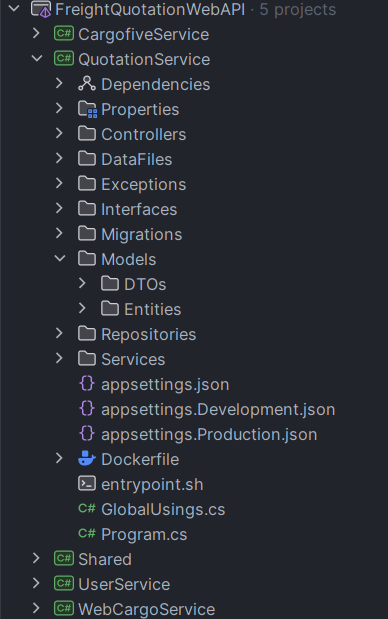
\includegraphics[width=0.5\linewidth]{images/ProjectStructure.png}
  \caption{\label{Figure:ProjectStructure}Project Structure}
\end{figure}

Besides the microservice components described in Section \ref{Section:Internal_Architecture_Microservices}, each microservice also contains other important directories and files, including:

\begin{description}
  \item[Dependencies] This directory contains all NuGet package dependencies required by the microservice.
  \item[DataFiles] This directory consists of miscellaneous data files. Quotation Service reads files in this directory to store initial data for locations and special handling codes, which are loaded into the database when the microservice starts for the first time.
  \item[Exceptions] This directory contains custom exception classes that represent specific error conditions in the microservice.
  \item[Interfaces] This directory contains interface definitions for Service and Repository modules. These interfaces define the contracts that implementing classes must adhere to, promoting loose coupling and easier testing.
  \item[Migrations] This directory holds the database migration files generated by .NET Entity Framework Core. These files define the changes to be applied to the database schema over time. When the database definition in the source code changes, a new migration file is created to represent the change. The database migration is applied before the microservice starts.
  \item[appsettings.json] This file contains configuration settings for the microservice, such as database connection strings and information related to the cloud platform components. There are also environment-specific versions of this file ("appsettings.Development.json" and "appsettings.Production.json") that specify additional settings when the microservice is running in a specific environment. These files do not contain secret values.
  \item[Dockerfile] This file defines the instructions to build a Docker image for the microservice. It specifies the base image, copies the source code, builds the project, and defines the entry point for running the microservice in a container.
  \item[entrypoint.sh] This script is executed when the microservice container starts. The microservice container has two distinct behaviors based on the parameters passed to this script. If the first parameter is "migrate", the script applies any pending database migrations and then exits. Otherwise, the script runs the microservice normally by executing the code defined in Program.cs.
  \item[Program.cs] This C\# file is responsible for configuring the web server, the middleware pipeline, and starting the web \ac{API}.
\end{description}

\subsection{Freight Rates and Quotes Obtainment}
\label{Subsection:Freight_Rates_And_Quotes_Obtainment}

When user makes a quote request to the web \ac{API}, it is routed to Quotation Service, which orchestrates the process by interacting with WebCargo Service and Cargofive Service.

Through configuration files, Quotation Service knows the addresses of WebCargo Service and Cargofive Service, which depend on whether the services are running in a local development environment or in an Azure production environment. Figures \ref{Figure:ServiceAddressesDevelopment} and \ref{Figure:ServiceAddressesProduction} show the addresses used in each environment. The addresses in a production environment are mapped to the full domain names of the services in the \ac{VNet} through \ac{DNS} records.

\begin{figure}[H]
  \centering
  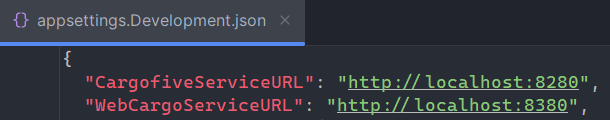
\includegraphics[width=0.8\linewidth]{images/ServiceAddressesDevelopment.png}
  \caption{\label{Figure:ServiceAddressesDevelopment}Service Addresses (Development Environment)}
\end{figure}

\begin{figure}[H]
  \centering
  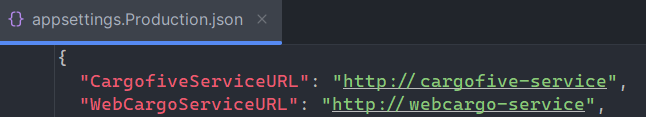
\includegraphics[width=0.8\linewidth]{images/ServiceAddressesProduction.png}
  \caption{\label{Figure:ServiceAddressesProduction}Service Addresses (Production Environment)}
\end{figure}

In this subsection, the process of obtaining an air freight quote is described. The process for sea freight quotes is analogous, with the only significant difference being that Cargofive Service is used instead of WebCargo Service.

When Quotation Service receives an air quote request from an end user, it is transformed into a \ac{DTO} corresponding to a C\# object shown in Figure \ref{Figure:AirQuoteRequestDTO}. If the \ac{DTO} is valid, Quotation Service sends a direct request to a WebCargo Service. This request comprises all the essential query parameters to search for air freight rates from the WebCargo \ac{API}: the \ac{IATA} codes of the origin and the destination airports. Quotation Service stores locations in its database, so it can retrieve the \ac{IATA} codes based on the location identifiers received in the air quote request. Quotation Service and WebCargo Service have an equivalent definition of the request \ac{DTO}, shown in Figure \ref{Figure:AirRateRequestDTO}. Figures \ref{Figure:AirQuoteRequestDTO}, \ref{Figure:AirRateRequestDTO}, and upcoming figures in this chapter contain blurred elements to hide irrelevant details.

\begin{figure}[H]
  \centering
  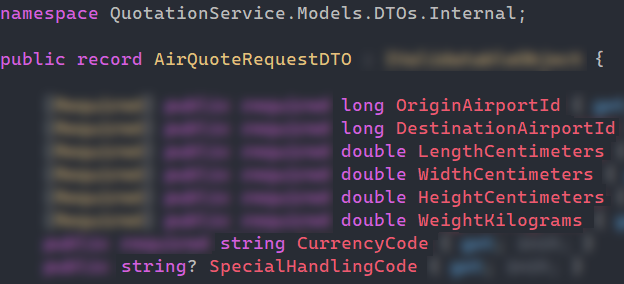
\includegraphics[width=0.7\linewidth]{images/AirQuoteRequestDTO.png}
  \caption{\label{Figure:AirQuoteRequestDTO}Air Quote Request DTO}
\end{figure}

\begin{figure}[H]
  \centering
  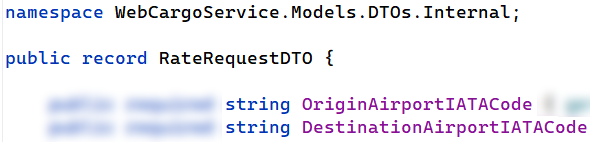
\includegraphics[width=0.7\linewidth]{images/AirRateRequestDTO.png}
  \caption{\label{Figure:AirRateRequestDTO}Air Rate Request DTO}
\end{figure}

When WebCargo Service receives the freight rate request, it checks if a valid cache entry exists for the given origin and destination. If it does, the cached freight rates are simply returned to Quotation Service as a list of \acp{DTO} shown in Figure \ref{Figure:AirRateDTO}.

If no valid cache entry exists, a request is made to the WebCargo \ac{API}. Once the response is received, its body containing the freight rates is deserialized into a list of \acp{DTO} with a structure similar to the WebCargo \ac{API}'s response body. Then, the retrieved freight rates are stored in the cache and sent to Quotation Service as previously described.

\begin{figure}[H]
  \centering
  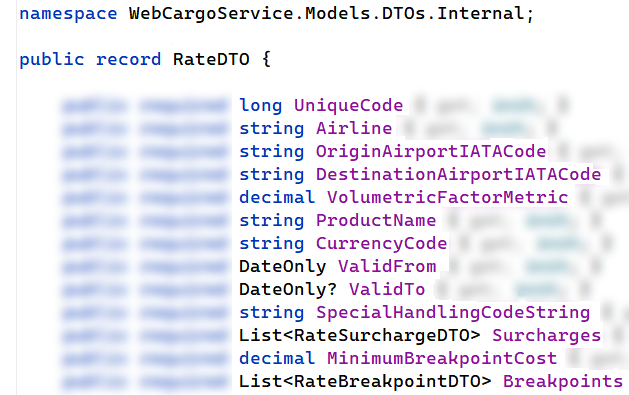
\includegraphics[width=0.75\linewidth]{images/AirRateDTO.png}
  \caption{\label{Figure:AirRateDTO}Air Rate DTO}
\end{figure}

Finally, Quotation Service works with the received freight rates to calculate freight quotes based on the user's input. The freight quote response is stored in the database and returned to the user as a \ac{DTO} shown in Figure \ref{Figure:AirQuoteResponseDTO}.

\begin{figure}[H]
  \centering
  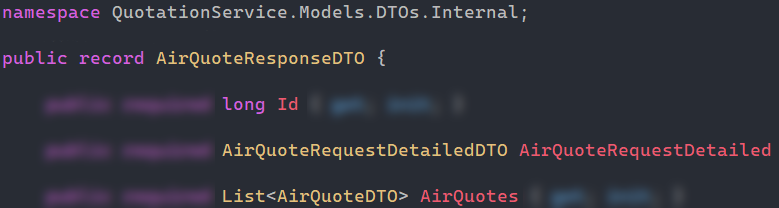
\includegraphics[width=0.9\linewidth]{images/AirQuoteResponseDTO.png}
  \caption{\label{Figure:AirQuoteResponseDTO}Air Quote Response DTO}
\end{figure}

The functionality described in this subsection can be tested in Postman. Figure \ref{Figure:AirQuoteRequestPostman} shows an example air quote request, where "baseUrl" is the \ac{URL} of the API Gateway. Figure \ref{Figure:AirQuoteResponsePostman} shows a part of the corresponding response.


\begin{figure}[H]
  \centering
  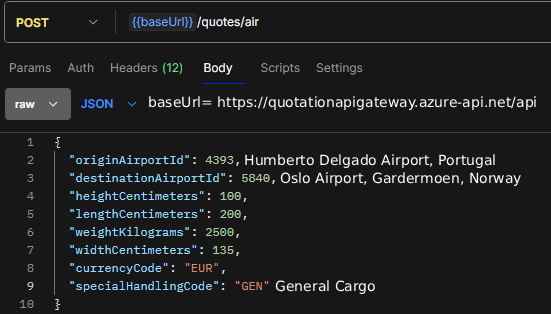
\includegraphics[width=0.9\linewidth]{images/AirQuoteRequestPostman.png}
  \caption{\label{Figure:AirQuoteRequestPostman}Air Quote Request in Postman}
\end{figure}

\begin{figure}[H]
  \centering
  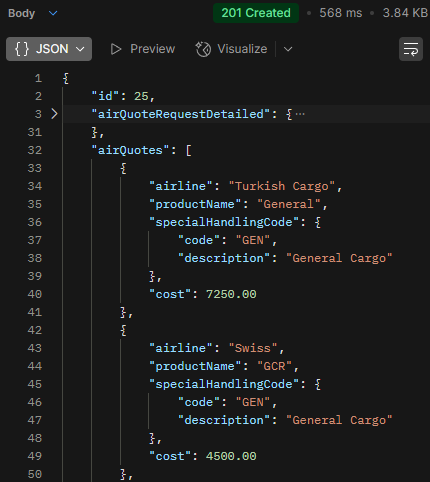
\includegraphics[width=0.8\linewidth]{images/AirQuoteResponsePostman.png}
  \caption{\label{Figure:AirQuoteResponsePostman}Air Quote Response in Postman}
\end{figure}

\subsection{Freight Rates Cache}
\label{Subsection:Freight_Rates_Cache}

External carrier \acp{API} impose rate limits on the number of requests that can be made within a specific time frame. To avoid exceeding these limits, freight rates obtained from the WebCargo and Cargofive \Acp{API} are cached for 1 day. The caching mechanism is implemented in WebCargo Service and Cargofive Service, respectively.

Each cache entry is based on a unique combination of request parameters that define what freight rates will be returned by the external carrier \ac{API}. For both \acp{API}, a combination of the origin and the destination locations is sufficient to uniquely identify a cache entry. When a request for freight rates is received, the service first checks if a valid cache entry exists. If it does, the cached freight rates are returned. If not, a request is made to the external carrier \ac{API}, and the retrieved freight rates are stored in the cache.

The main purpose of the caching mechanism is to reduce the number of requests to the external carrier \acp{API}. Because of this, the databases of WebCargo Service and Cargofive Service store not only the rate history, but also the cached data, for simplicity. However, this implementation has some drawbacks, such as increased cached lookup times and potential database load. In future work, a dedicated caching alternative would be useful for its increased performance and built-in cache expiration mechanisms.

\subsection{Quote History}
\label{Subsection:Quote_History}

Whenever Quotation Service processes a freight quote request, it stores the request and response data in its database. This allows users to retrieve their quotation history through a dedicated endpoint.

The returned history is ordered from newest to oldest and paginated to limit the number of results in a single response. Pagination parameters are specified in the request query string. The parameter "page" indicates the page number, while "limit" indicates the number of results per page. If these parameters are not specified, default values are used (1 for page and 100 for limit).

Figure \ref{Figure:QuoteHistoryRequestPostman} shows an example request to the quote history endpoint in Postman. Figure \ref{Figure:QuoteHistoryResponsePostman} shows the corresponding response, which was collapsed for visibility.

\begin{figure}[H]
  \centering
  
\includegraphics[width=0.8\linewidth]{images/QuoteHistoryRequestPostman.png}
  \caption{\label{Figure:QuoteHistoryRequestPostman}Quote History Request in Postman}
\end{figure}


\begin{figure}[H]
  \centering
  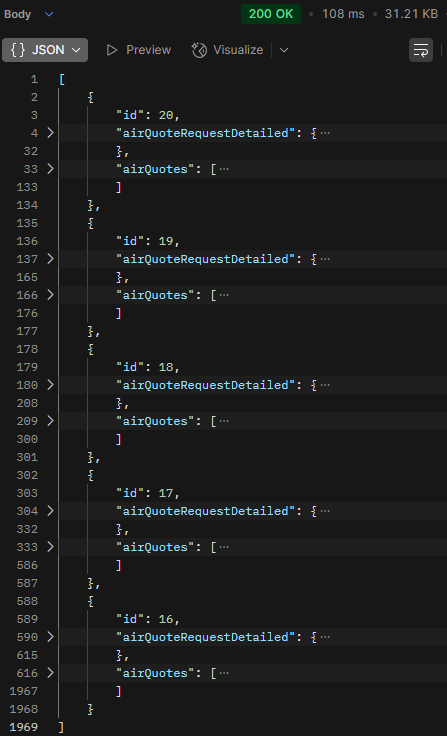
\includegraphics[width=0.7\linewidth]{images/QuoteHistoryResponsePostman.png}
  \caption{\label{Figure:QuoteHistoryResponsePostman}Quote History Response in Postman}
\end{figure}

\subsection{Location Search}
\label{Subsection:Location_Search}

Quotation Service exposes an endpoint that allows users to search for locations by name. This functionality is useful when users need to find the identifier of a location to use in a freight quote request.

The location search endpoint accepts a query parameter for the location name and another for the location type. Furthermore, it supports pagination, similarly to the one described in Subsection \ref{Subsection:Quote_History}. The endpoint returns a list of matching locations with their identifiers and other information.

Figure \ref{Figure:LocationSearchRequestPostman} shows an example request to the endpoint in Postman for airport locations whose name contains "barce". Figure \ref{Figure:LocationSearchResponsePostman} shows the resulting response.

\begin{figure}[H]
  \centering
  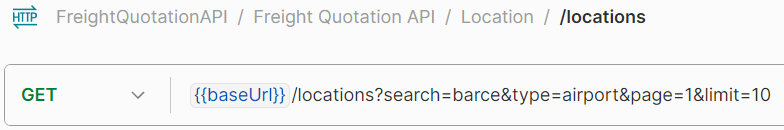
\includegraphics[width=0.9\linewidth]{images/LocationSearchRequestPostman.png}
  \caption{\label{Figure:LocationSearchRequestPostman}Location Search Request in Postman}
\end{figure}

\begin{figure}[H]
  \centering
  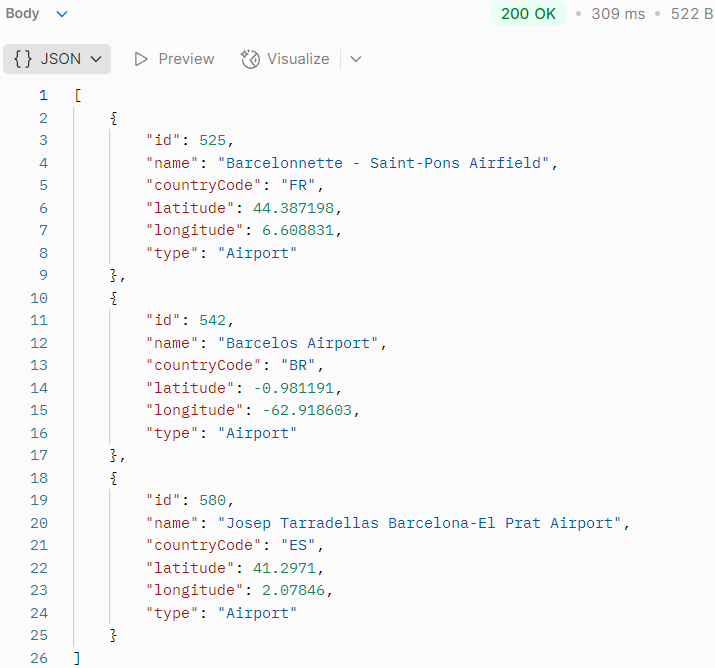
\includegraphics[width=0.8\linewidth]{images/LocationSearchResponsePostman.png}
  \caption{\label{Figure:LocationSearchResponsePostman}Location Search Response in Postman}
\end{figure}

\subsection{\texorpdfstring{\ac{RBAC}}{RBAC}}
\label{Subsection:RBAC}

The microservices rely on the authentication verification performed by the \ac{API} Gateway. Therefore, they do not need to validate access tokens themselves. Still, they must enforce authorization policies to restrict access to resources based on user roles or more complex business rules.

Only users with the "Administrator" role can access the endpoint to search for other users in the system. User roles can be found in the "roles" claim of the access token (\ac{JWT}). User roles can be assigned manually through the Azure portal. Alternatively, User Service can assign roles by calling the appropriate Graph \ac{API}\footnote{Microsoft Learn, "Use the Microsoft Graph API", \url{https://learn.microsoft.com/en-us/graph/use-the-api}, (accessed 15 Sep. 2025)} endpoint, which is used to interact with Microsoft's cloud resources.

Figure \ref{Figure:UserSearchRequestPostman} shows a search request in Postman for users whose name contains "mar". Figure \ref{UserSearchResponsePostmanForbidden} shows the "403 Forbidden" response received when the request is made with a \ac{JWT} of a user without the "Administrator" role. Conversely, Figure \ref{UserSearchResponsePostmanSuccess} shows the successful response received when the request is made with a \ac{JWT} of an administrator.

\begin{figure}[H]
  \centering
  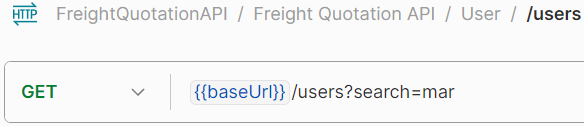
\includegraphics[width=0.7\linewidth]{images/UserSearchRequestPostman.png}
  \caption{\label{Figure:UserSearchRequestPostman}User Search Request in Postman}
\end{figure}

\begin{figure}[H]
  \centering
  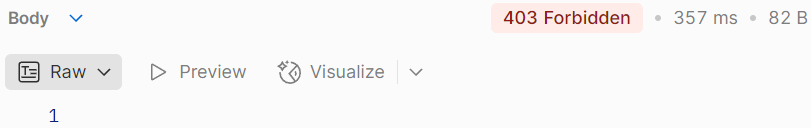
\includegraphics[width=0.9\linewidth]{images/UserSearchResponsePostmanForbidden.png}
  \caption{\label{UserSearchResponsePostmanForbidden}User Search Response in Postman (Access Forbidden)}
\end{figure}

\begin{figure}[H]
  \centering
  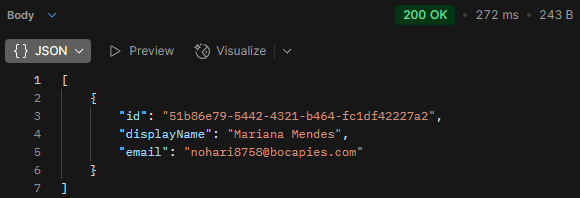
\includegraphics[width=0.9\linewidth]{images/UserSearchResponsePostmanSuccess.png}
  \caption{\label{UserSearchResponsePostmanSuccess}User Search Response in Postman (Success)}
\end{figure}

\subsection{User Data Deletion}
\label{Subsection:User_Data_Deletion}

When a user is deleted, all their associated data is also deleted from the web \ac{API}'s databases. Since Entra ID is the Identity Provider, it is responsible for managing user accounts. Therefore, User Service must be informed about user account deletions by communicating with Entra ID. In Subsection \ref{Subsection:Event_Driven_Inter_Service_Communication}, two possible approaches to get this information were mentioned: subscribing to the Identity Provider's user deletion notifications, or polling the Identity Provider periodically. Entra ID supports both approaches through the Microsoft Graph \ac{API}.

The first approach involves subscribing to Microsoft Graph \ac{API}'s change notifications for user deletions. This requires setting up a webhook endpoint in User Service to receive notifications, which Entra ID communicates with. However, the Graph \ac{API} only supports this approach for workforce tenants, which are intended for employees of an organization. The implemented web \ac{API} is intended for general customer users and thus utilizes a different tenant type. Therefore, this event-driven approach is not feasible for the web \ac{API}.

The second approach involves polling the Microsoft Graph \ac{API}. Indiscriminate polling would be inefficient, as it would involve returning all users and checking for deletions. Instead, User Service uses delta queries\footnote{Microsoft Learn, "Use delta query to track changes in Microsoft Graph data", \url{https://learn.microsoft.com/en-us/graph/delta-query-overview}, (accessed 15 Sep. 2025)} to retrieve only the changes that occurred since the last query. This is achieved by storing a delta link provided by the Graph \ac{API} after each query in the User Service's database. The delta link is then used in subsequent queries to fetch only the changes since the last query. User Service polls the Graph \ac{API} every 15 minutes.

When User Service retrieves at least one deleted user through polling, it sends a batch of messages to a Service Bus (Message Broker) topic called "user\_deleted". Each message contains the identifier of a deleted user. Any microservice may subscribe to this topic. In particular, Quotation Service has a subscription to this topic and processes each message by deleting the quote history of the corresponding user from its database.

\section{Cloud Components Configuration}

\subsection{API Gateway Configuration}
\label{Subsection:API_Gateway_Configuration}

An Azure \ac{API} Management instance is used to route incoming requests to the appropriate microservice, thus acting as the \ac{API} Gateway. A single \ac{API} is added to the \Ac{API} Management instance by importing the definition from the OpenAPI specification file mentioned in Section \ref{Section:API_Specification}. This \ac{API} is named "Freight Quotation API".

The Freight Quotation \ac{API} has a "Settings" tab, shown in Figure \ref{Figure:APIGatewaySettings}, where general configurations are made. Secure \ac{HTTP} access is enforced by allowing only \ac{HTTPS} requests. Furthermore, the base public \ac{URL} is defined ("https://quotationapigateway.azure-api.net/api"), which clients must use to access the web \ac{API}.

\begin{figure}[H]
  \centering
  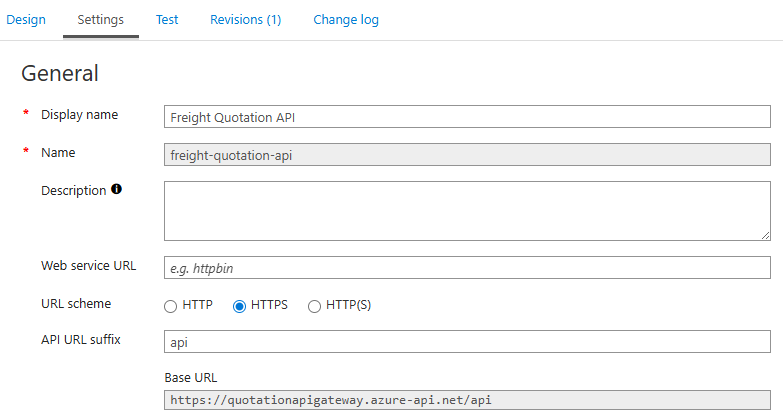
\includegraphics[width=0.9\linewidth]{images/APIGatewaySettings.png}
  \caption{\label{Figure:APIGatewaySettings}API Gateway Settings}
\end{figure}

Unlike the microservice components, the \ac{API} Gateway accepts communication from the public internet, as it resides in a subnet that allows such traffic. The microservices, which reside in a different subnet, rely on the \ac{API} Gateway to interact with the Client. Because of this, each microservice is added as a separate backend service to the \ac{API} Gateway, as shown in Figure \ref{Figure:APIGatewayBackends}. The "Backend name" is used as a simple alias to identify the backend service. The "Run URL" is the internal \ac{URL} of the microservice in the \ac{VNet}.

\begin{figure}[H]
  \centering
  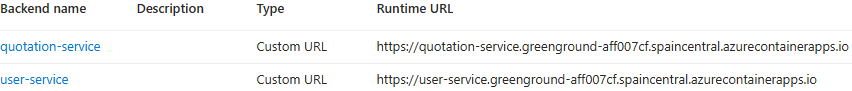
\includegraphics[width=0.9\linewidth]{images/APIGatewayBackends.png}
  \caption{\label{Figure:APIGatewayBackends}API Gateway Backends}
\end{figure}

The \ac{API} Gateway's behavior towards the Freight Quotation API is defined in the "Design" tab. In this tab, an \ac{XML} configuration file defines multiple policies that are applied to incoming requests or outgoing responses. Considering the roles of the \ac{API} Gateway mentioned in Subsection \ref{Subsection:API_Gateway}, the policies can be split into three parts: \Ac{CORS}, authentication, and routing.

\ac{CORS} policies are applied to all incoming requests to allow cross-origin requests from the Client. Since the Client application does not have a fixed domain name, the \ac{CORS} policy allows requests from any origin and accepts any \ac{HTTP} method. However, if the Client had a fixed domain name, the \ac{CORS} policy would be more restrictive. The \ac{CORS} policy is shown in Figure \ref{Figure:APIGatewayConfigurationCORS}.

\begin{figure}[H]
  \centering
  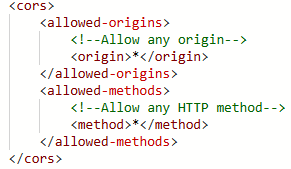
\includegraphics[width=0.4\linewidth]{images/APIGatewayConfigurationCORS.png}
  \caption{\label{Figure:APIGatewayConfigurationCORS}API Gateway \ac{CORS} Policy}
\end{figure}

The next step is to enforce authentication by validating the access token (\ac{JWT}) included in the "Authorization" header of incoming requests. The \ac{API} Gateway uses the OpenID Connect metadata document of the Identity Provider to validate the token's signature and claims. If the token is invalid or missing, the request is rejected with a "401 Unauthorized" response. Figure \ref{Figure:APIGatewayConfigurationAuthentication} displays the authentication policy configuration with explanatory comments.

\begin{figure}[H]
  \centering
  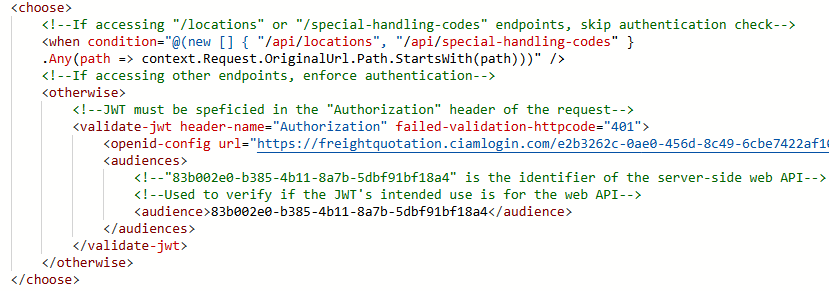
\includegraphics[width=0.9\linewidth]{images/APIGatewayConfigurationAuthentication.png}
  \caption{\label{Figure:APIGatewayConfigurationAuthentication}API Gateway Authentication Policy}
\end{figure}

Finally, the \ac{API} Gateway routes incoming requests to the appropriate microservice based on the request's destination. The routing policy is shown in Figure \ref{Figure:APIGatewayConfigurationRouting}. The policy uses the backend identifier of each backend service defined in Figure \ref{Figure:APIGatewayBackends} to identify the target microservice.

\begin{figure}[H]
  \centering
  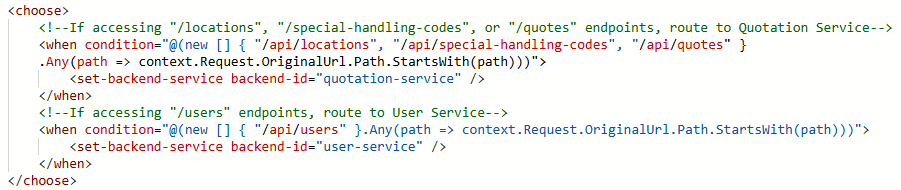
\includegraphics[width=1\linewidth]{images/APIGatewayConfigurationRouting.png}
  \caption{\label{Figure:APIGatewayConfigurationRouting}API Gateway Routing Policy}
\end{figure}

\subsection{Microservice Environment Configuration}
\label{Subsection:Microservice_Environment_Configuration}

The Azure Container Apps Environment hosts all microservices as Azure Container Apps. In addition, there is one Container App Job for each microservice, which is used to apply database migrations when a new deployment occurs. The Container Apps Environment resides within a dedicated subnet ("ContainerEnvironmentSubnet") in the \ac{VNet} to ensure secure communication. This subnet adheres to the default Azure subnet policies, which only allow traffic from other components within the \ac{VNet}, or private endpoints. Figure \ref{Figure:ContainerAppsEnvironment} shows the overall configuration of the Container Apps Environment.

\begin{figure}[H]
  \centering
  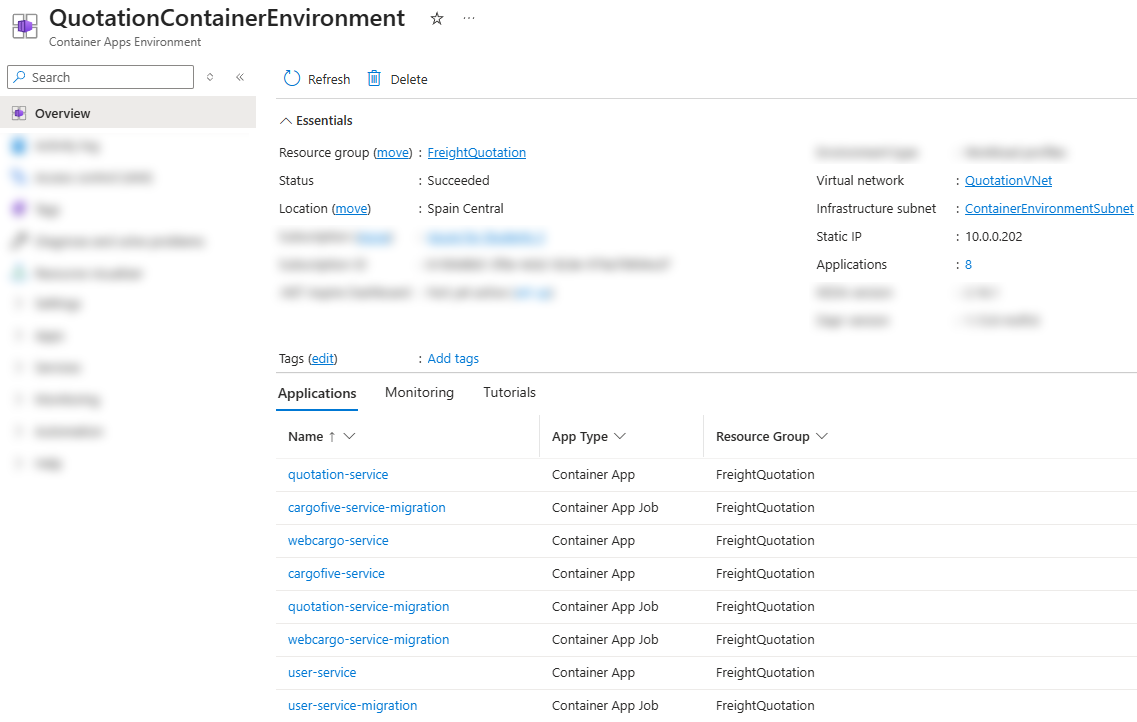
\includegraphics[width=1\linewidth]{images/ContainerAppsEnvironment.png}
  \caption{\label{Figure:ContainerAppsEnvironment}Container Apps Environment Configuration}
\end{figure}

Each microservice is deployed as a separate Container App. Each Container App runs a specific Docker image version stored in the Container Registry. When the \ac{CI/CD} pipeline deploys a new version of a microservice, it updates the Container App to use the new Docker image, creating a revision of the Container App. Microservices run in Docker containers of that image. Each microservice instance has 0.5 general-purpose \acp{vCPU} and 1 \ac{GiB} of memory allocated.

Another valuable feature is the ability to set scaling rules for each microservice, which can be based on \ac{HTTP} traffic, \ac{CPU} usage, or memory usage. Specifically, every Container App is configured to scale between 1 and 10 instances, based on the average number of concurrent \ac{HTTP} requests being processed per instance. If this number exceeds 50, the Container App will automatically scale up to deal with the increased load. Conversely, if the average workload remains lower for 5 minutes, the Container App will scale down to conserve resources. Figure \ref{Figure:ContainerAppsScaling} shows the scaling configuration.

\begin{figure}[H]
  \centering
  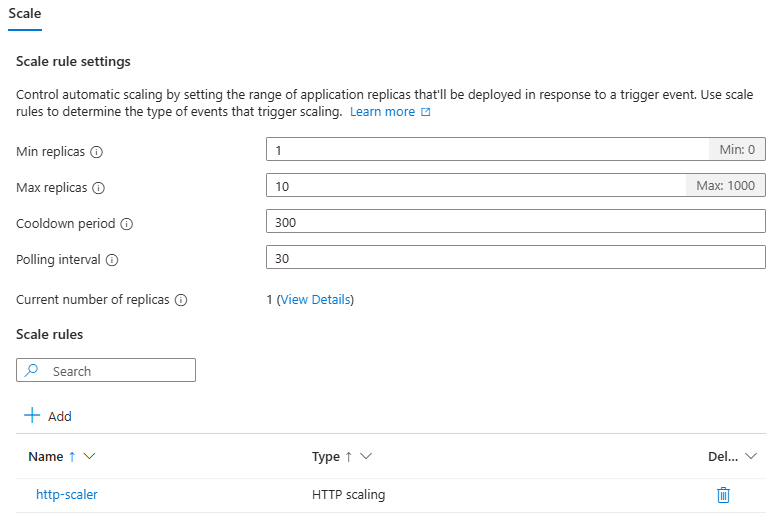
\includegraphics[width=0.9\linewidth]{images/ContainerAppsScaling.png}
  \caption{\label{Figure:ContainerAppsScaling}Container App Scaling Rules}
\end{figure}

\subsection{Data Persistence Layer Configuration}

An Azure SQL Server instance hosts the databases of all microservices. Each microservice has its own SQL database. Public access to the SQL Server is disabled, so the server can only be accessed from within the \ac{VNet} through a private endpoint.

Every microservice connects to its database through passwordless authentication, allowing Container Apps to authenticate without storing confidential connection strings. Instead, a generic connection string that depends only on the name of the target database is enough. To achieve this, each Container App is assigned a managed identity, which is then granted the "db\_datareader" and "db\_datawriter" roles in the target database. Figure \ref{Figure:DatabaseConfigurationManagedIdentity} shows the active managed identity of WebCargo Service's Container App, which is similar for all other microservices.
Figure \ref{Figure:DatabaseConfigurationQuery} demonstrates the subsequent step, where a \ac{SQL} query executed in the Azure Portal to assign the necessary database roles.

\begin{figure}[H]
  \centering
  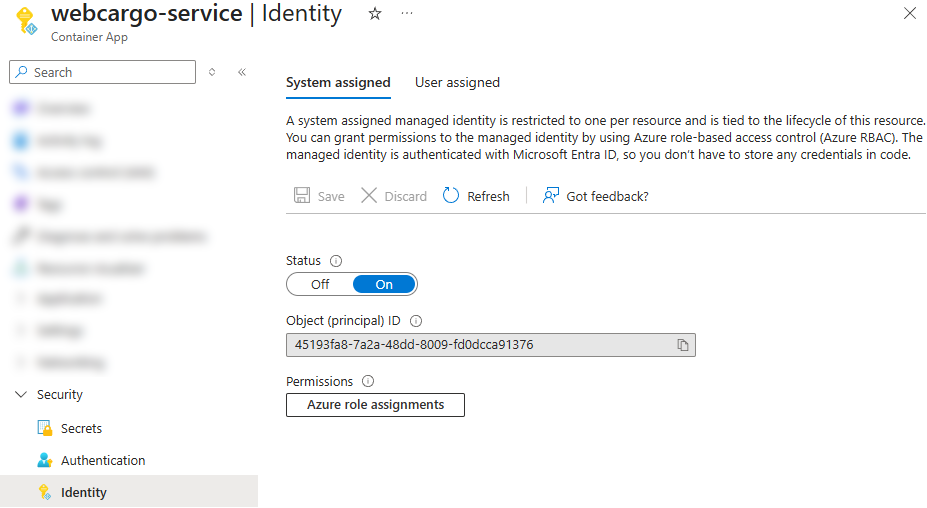
\includegraphics[width=0.9\linewidth]{images/DatabaseConfigurationManagedIdentity.png}
  \caption{\label{Figure:DatabaseConfigurationManagedIdentity}Container App's Managed Identity}
\end{figure}

\begin{figure}[H]
  \centering
  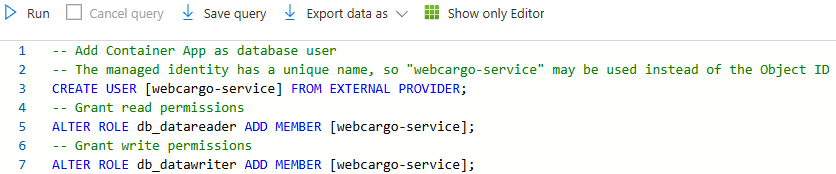
\includegraphics[width=1\linewidth]{images/DatabaseConfigurationQuery.png}
  \caption{\label{Figure:DatabaseConfigurationQuery}Database Roles Assignment}
\end{figure}

Different databases may have differing computation power and storage capacity, depending on the microservice's needs. All databases have 16 \acp{GB} of storage, to save costs. In terms of computation power, Quotation Service's database has 2 general-purpose \acp{vCPU}, while the other microservices' databases have the default 1 \ac{vCPU}. This disparity is due to the fact that this database will be used in performance testing. Figure \ref{Figure:DatabaseConfigurationBase} shows the basic configuration properties of the Quotation Service's database, which is similar to all others, barring the number of \acp{vCPU}.

\begin{figure}[H]
  \centering
  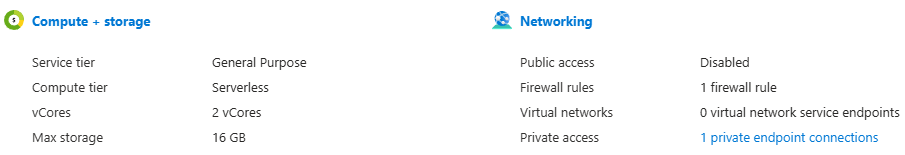
\includegraphics[width=0.9\linewidth]{images/DatabaseConfigurationBase.png}
  \caption{\label{Figure:DatabaseConfigurationBase}SQL Databases Base Configuration}
\end{figure}

\subsection{Secret Storage Configuration}

For security reasons, the source code of each microservice does not contain any secret values. Instead, Azure Key Vault is used to securely store confidential information for production environments, which is made available to the microservices through a private endpoint. The Key Vault stores the \ac{API} keys to authenticate with external carrier \acp{API}, the Service Bus connection string, and the secret to access Entra ID's resources. Figure \ref{Figure:KeyVaultSecrets} enumerates the names of all secrets.

\begin{figure}[H]
  \centering
  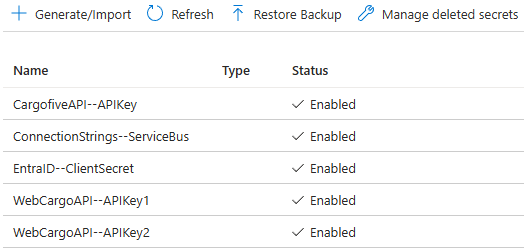
\includegraphics[width=0.8\linewidth]{images/KeyVaultSecrets.png}
  \caption{\label{Figure:KeyVaultSecrets}Key Vault Secrets}
\end{figure}

\section{\texorpdfstring{\ac{CI/CD}}{CI/CD} Pipeline Configuration}

The Code Repository, which is hosted on GitHub, includes a directory named ".github" containing all \ac{CI/CD} pipeline configuration files in the "workflows" subdirectory. Each workflow file is associated with a specific microservice. This directory also contains Shell script files in the "scripts" subdirectory that are used as part of the workflows. Figure \ref{Figure:GithubScriptsAndWorkflows} presents the structure of the ".github" directory.

\begin{figure}[H]
  \centering
  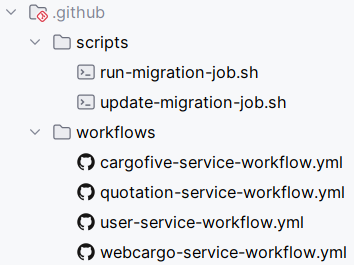
\includegraphics[width=0.5\linewidth]{images/GithubScriptsAndWorkflows.png}
  \caption{\label{Figure:GithubScriptsAndWorkflows}Github Scripts and Workflows}
\end{figure}

The workflow file related to Quotation Service will be explained, as an example. The workflows of the other microservices follow equivalent steps.

The beginning of the workflow file defines its name, what conditions trigger its execution, and the environment variables it uses. This particular workflow is triggered when a change that affects either the "QuotationService" or "Shared" root directories is pushed to the master branch. The environment variables include Azure-related values and the name of the root folder of the microservice. Figure \ref{Figure:GithubWorkflowHeader} shows this part of the workflow file.

\begin{figure}[H]
  \centering
  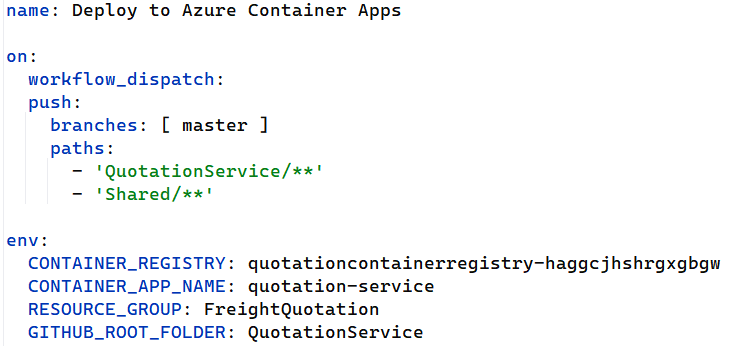
\includegraphics[width=0.9\linewidth]{images/GithubWorkflowHeader.png}
  \caption{\label{Figure:GithubWorkflowHeader}Workflow Header}
\end{figure}

The latest version of Ubuntu is set as the \ac{OS} of the workflow runner. The first two steps of the workflow are preparatory and do not interact with Azure yet. The first step checks out the source code of the repository, making it available to the workflow runner. The second step sets up Docker functionality. Figure \ref{Figure:GithubWorkflowPreparation} shows these steps.

\begin{figure}[H]
  \centering
  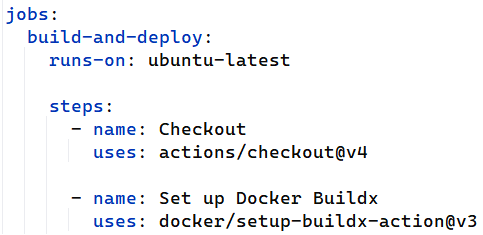
\includegraphics[width=0.6\linewidth]{images/GithubWorkflowPreparation.png}
  \caption{\label{Figure:GithubWorkflowPreparation}Workflow Preparation Steps}
\end{figure}

The objectives of the subsequent two steps are to build and push the new Docker image of the microservice to the Container Registry. The first step logs into the Container Registry using the "docker/login-action" action. This step uses Azure credentials stored in the repository's secrets to authenticate. The second step builds the Docker image according to the Dockerfile present in the directory of the microservice. Then, the workflow runner tags the Docker image with the current commit hash and pushes it to the Container Registry. Figure \ref{Figure:GithubWorkflowContainerRegistry} shows these steps.

\begin{figure}[H]
  \centering
  \includegraphics[width=1\linewidth]{images/GithubWorkflowContainerRegistry.png}
  \caption{\label{Figure:GithubWorkflowContainerRegistry}Workflow Docker Build and Push Steps}
\end{figure}

The next step logs into the Azure account of the web \ac{API}'s resources, which is a prerequisite for the upcoming steps. To authenticate, it uses credentials stored in the Github repository's secrets. Figure \ref{Figure:GithubWorkflowAzureLogin} illustrates this step.

\begin{figure}[H]
  \centering
  \includegraphics[width=0.6\linewidth]{images/GithubWorkflowAzureLogin.png}
  \caption{\label{Figure:GithubWorkflowAzureLogin}Workflow Azure Login Step}
\end{figure}

Once the workflow runner logs into the Azure account, it executes the Shell script named "update-migration.job.sh". This script updates the Container App Job of the microservice to use the new Docker image. This is essential to ensure that the database migration is applied using the latest version of the microservice. Figure \ref{Figure:GithubWorkflowMigrationJobUpdate} shows this step.

\begin{figure}[H]
  \centering
  \includegraphics[width=0.6\linewidth]{images/GithubWorkflowMigrationJobUpdate.png}
  \caption{\label{Figure:GithubWorkflowMigrationJobUpdate}Workflow Migration Job Update Step}
\end{figure}

The following step executes the Shell script named "run-migration-job.sh". This script starts a new instance of the Container App Job, which applies any pending database migrations to the microservice's associated database. The script then waits for the job to complete successfully before proceeding by periodically checking the execution status. Figure \ref{Figure:GithubWorkflowMigrationJobExecution} shows this step.

\begin{figure}[H]
  \centering
  \includegraphics[width=0.6\linewidth]{images/GithubWorkflowMigrationJobExecution.png}
  \caption{\label{Figure:GithubWorkflowMigrationJobExecution}Workflow Migration Job Execution Step}
\end{figure}

The last step deploys the Docker image that was pushed to the Container Registry to the Container App associated with the microservice. This effectively updates the running instance of the microservice to the latest version. Figure \ref{Figure:GithubWorkflowContainerAppDeployment} shows this step.

\begin{figure}[H]
  \centering
  \includegraphics[width=1\linewidth]{images/GithubWorkflowContainerAppDeployment.png}
  \caption{\label{Figure:GithubWorkflowContainerAppDeployment}Workflow Container App Deployment Step}
\end{figure}

\chapter{Evaluation}
\label{Chapter:Evaluation}

This chapter analyses the quality of the web \ac{API} implemented in Chapter \ref{Chapter:Implementation} in terms of reliability and performance. It also offers the necessary information to estimate the cost of the proposed solution in a real-world scenario. Afterwards, the extent to which the web \ac{API} satisfies the requirements enumerated in Chapter \ref{Section:Requirements} is evaluated.

\section{Testing Strategy}
\label{Section:Testing_Strategy}

Unit tests and integration tests are important to ensure the quality of the microservices' source code by automatically verifying their correctness. In the implemented web \ac{API}, unit tests aim to verify individual microservice components in isolation. On the other hand, integration tests focus on the communication with other microservices, cloud components, or external \acp{API}. Furthermore, testing can be added as a step of the CI/CD pipeline to ensure that changes do not introduce bugs.

However, due to time constraints, the implementation of automated tests was not feasible. Therefore, the testing strategy for the web \ac{API} relied solely on manual testing. Manual testing was performed using Postman, as demonstrated in Section \ref{Section:Microservices_Implementation}. Postman was used to test all endpoints of the web \ac{API}, including various scenarios that encompassed valid requests, invalid requests, and edge cases. In addition, database records were inspected directly in the Azure Portal to verify that data was being stored as intended.

\section{Cost Analysis}
\label{Section:Cost_Analysis}

\subsection{Cost Analysis Context}
\label{Subsection:Cost_Analysis_Context}

Hosting software components on a cloud platform incurs costs. During the development of the web \ac{API}, free Azure subscriptions with limited budgets were used.

Cloud platforms offer multiple pricing tiers for their cloud services. Pricing tiers focused on development and testing were selected to minimize costs while still providing the necessary features. However, these pricing tiers are not suitable for enterprise production environments, as they have lower limits in terms of performance, scalability, and availability.

Determining concrete monetary values for the cost of hosting the web \ac{API} is beyond the scope of this dissertation. The goal of the cost analysis is to provide the necessary parameters to estimate the cost of hosting and running the web \ac{API} in a real-world production environment.

Each cloud platform has distinct pricing models for its services. This Section estimates and compares the cost of hosting the web \ac{API} in three major cloud platforms: Microsoft Azure, \ac{AWS}\footnote{Amazon Web Services, \url{https://aws.amazon.com/}, (accessed 21 Sep. 2025)}, and \ac{GCP}\footnote{Google Cloud Platform, \url{https://cloud.google.com/}, (accessed 21 Sep. 2025)}. To simplify, the cost analysis focuses on the most expensive components of the web \ac{API}. The most expensive components are the \ac{API} Gateway, the Microservice Environment, and the Data Persistence Layer. Together, they contribute to over 90\% of the total cost. This conclusion was reached by examining two main sources: the official pricing documentation for each cloud provider, and the expenditure data from the development phase of the web \ac{API}.

Table \ref{Table:CloudPlatformsServiceMapping} summarizes the mapping of web \ac{API} components to their respective cloud platform services considered for the cost analysis.

\begin{table}[h!]
  \centering
  \begin{tabular}{|M{135pt}|M{80pt}|M{80pt}|M{80pt}|}
    \hline
    \multicolumn{1}{|c|}{\textbf{Web \ac{API} Component}} & \multicolumn{1}{c|}{\textbf{Azure}} & \multicolumn{1}{c|}{\textbf{\ac{AWS}}} & \multicolumn{1}{c|}{\textbf{\ac{GCP}}} \\
    \hline
    \ac{API} Gateway                                      & API Management                      & API Gateway                            & API Gateway                            \\
    \hline
    Microservice Environment                              & Container Apps Environment          & \ac{ECS}                               & Cloud Run                              \\
    \hline
    Data Persistence Layer                                & SQL Server                          & \ac{RDS} for SQL Server                & Cloud SQL with SQL Server              \\
    \hline
  \end{tabular}
  \vspace{10pt}
  \caption{Cloud Platform Service Mapping}
  \label{Table:CloudPlatformsServiceMapping}
\end{table}

\subsection{Cost Analysis Parameters}
\label{Subsection:Cost_Analysis_Parameters}

The total cost of hosting the web \ac{API} depends on various parameters, so it is difficult to estimate the cost accurately. Still, the parameters were selected based on the requirements defined in Section \ref{Section:Requirements}, the results of the performance test in Subsection \ref{Subsection:Performance_Test_Results_and_Analysis}, and mid-tier pricing plans on the cloud platforms.

Table \ref{Table:Cost_Analysis_Parameters} lists all parameters considered in the cost analysis, along with the rationale behind their values.

\begin{longtable}{|M{70pt}|M{55pt}|m{300pt}|}

  \caption{Cost Analysis Parameters}
  \label{Table:Cost_Analysis_Parameters}                                                                                                                                                                                                                                                                                                                                                                                                                                                 \\

  \hline
  \multicolumn{1}{|c|}{\textbf{Parameter}}
   & \multicolumn{1}{c|}{\textbf{Value}}
   & \multicolumn{1}{c|}{\textbf{Rationale}}
  \endfirsthead

  \hline
  \multicolumn{1}{|c|}{\textbf{Parameter}}
   & \multicolumn{1}{c|}{\textbf{Value}}
   & \multicolumn{1}{c|}{\textbf{Rationale}}                                                                                                                                                                                                                                                                                                                                                                                                                                             \\
  \hline
  \endhead

  \hline
  \multicolumn{3}{r}{\textit{Continued on the next page...}}                                                                                                                                                                                                                                                                                                                                                                                                                             \\
  \endfoot

  \hline
  \endlastfoot
  \hline
  API Requests (Monthly)
   & 100 Million
   & Represents 38.6 user requests per second, on average. This value considers the performance test described in Section \ref{Section:Performance_Evaluation}, where the web \ac{API} dealt with 400 requests per second. However, that value is intended to represent a surge in traffic, and does not take into account quotation requests, which are much more complex. Therefore, a much lower value was chosen.                                                                    \\
  \hline
  Data Egress (Monthly)
   & 500 GB
   & Considering value of the "API Requests (Monthly)" parameter, this amounts to an average of 5 \ac{KB} per request response. The size of the responses delivered to users varies heavily, ranging from less than 1 \ac{KB}, to more than 100 \ac{KB} for some quote history requests. 5 \ac{KB} represents a typical quote request response size.                                                                                                                                     \\

  \hline
  Virtual Network Integration
   & Yes
   & The \ac{API} Gateway must integrate with the \ac{VNet}, as implemented in the web \ac{API}. Therefore, \ac{VNet} integration costs are considered.                                                                                                                                                                                                                                                                                                                                  \\
  \hline
  Number of Microservices
   & 4
   & As implemented in the web \ac{API}.                                                                                                                                                                                                                                                                                                                                                                                                                                                 \\
  \hline
  Microservice CPU (Average)
   & 2 vCPUs
   & This value assumes each microservice has 4 active instances with 0.5 \acp{vCPU}, on average. All chosen cloud platform \acp{vCPU} belong to a general-purpose tier, although their processing power may still vary between cloud providers.                                                                                                                                                                                                                                         \\
  \hline
  Microservice Memory (Average)
   & 4 GiB
   & This value assumes that, on average, each microservice has 4 instances with 1 \ac{GiB} of memory running.                                                                                                                                                                                                                                                                                                                                                                           \\
  \hline
  Number of Databases
   & 3
   & User Service's database has extremely low resource requirements. Therefore, only Quotation Service, WebCargo Service, and Cargofive Service's databases were considered.                                                                                                                                                                                                                                                                                                            \\
  \hline
  Database CPU (Static)
   & 4 vCPUs
   & It is difficult to predict the necessary \ac{CPU} resources for the databases. Quotation requests involve more resource-intensive queries than the ones used in the performance test, so more than 2 \acp{vCPU} were selected. The value of this parameter is also associated with mid-tier options in cloud provider offerings. For easier comparison between cloud providers, the database \ac{CPU} allocation is static, as opposed to being dynamically adjusted based on load. \\
  \hline
  Database Memory (Static)
   & 16 GiB
   & This value is in line with cloud provider options offering 4 \acp{vCPU}.                                                                                                                                                                                                                                                                                                                                                                                                            \\
  \hline
  Database Storage (Static)
   & 128 GB
   & The database storage requirements are hard to predict without real usage data. This value coincides with mid-tier options in cloud provider offerings.                                                                                                                                                                                                                                                                                                                              \\
  \hline
  Payment Commitment Length
   & 1 Year
   & For lower costs and easier comparison between cloud providers.                                                                                                                                                                                                                                                                                                                                                                                                                      \\
  \hline
  Deployment Region
   & Paris, France
   & Cheaper than most other European regions and supports most offerings.                                                                                                                                                                                                                                                                                                                                                                                                               \\
  \hline
  User Traffic Origin
   & Europe
   & Applies to all requests, to simplify analysis.                                                                                                                                                                                                                                                                                                                                                                                                                                      \\
\end{longtable}

\section{Performance Evaluation}
\label{Section:Performance_Evaluation}

\subsection{Performance Test Scenario}
\label{Subsection:Performance_Test_Scenario}

A performance evaluation was performed to analyze the responsiveness of the web \ac{API} under the conditions specified by Requirement \ref{Requirement:10}. To do so, a test scenario was designed and executed with the goal of testing the base performance of the system.

The test scenario consists of simulating 200 concurrent users send GET requests the "locations/\{id\}" endpoint. This involves 200 users sending requests simultaneously to the web \ac{API}, waiting for a response, and then immediately sending another request once a response is received. This process lasts 3 minutes, with a previous warm-up period of 2 minutes. The warm-up period is important to allow the necessary microservice replicas to be created and initialized before real measurements are considered. The location identifier used for all requests is "1234", which corresponds to an airport location stored in Quotation Service's database. Neither the \ac{API} Gateway nor Quotation Service have any caching mechanism for endpoint requests, so that every request is processed from scratch.

To satisfy Requirement \ref{Requirement:10}, the 90th percentile of response times must be under 500 milliseconds. This means that at least 90\% of all requests must receive a response in less than 500 milliseconds. Considering that the scenario involves 200 concurrent users, the web \ac{API} must be able to handle at least 400 requests of this type per second, on average. Equation \ref{Equation:Requests_Per_Second} shows how this value is calculated.

\begin{equation}
  \text{Requests (per second)} = \frac{\text{Concurrent users}}{\text{Response time (seconds)}}
  \label{Equation:Requests_Per_Second}
\end{equation}

\vspace{10pt}

\subsection{Performance Test Setup and Configuration}
\label{Subsection:Performance_Test_Setup_and_Configuration}

The Azure Portal provides a service called "Azure Load Testing" that allows the creation and execution of performance test scenarios. This service was used to set up and run the performance test scenario described in Subsection \ref{Subsection:Performance_Test_Scenario}.

The performance test is an Azure "URL-based test" where a specific public endpoint of the web \ac{API} is targeted. This \ac{URL} is shown in Figure \ref{Figure:LoadTestingRequestSpecification}, along with other configuration parameters.

\begin{figure}[H]
  \centering
  \includegraphics[width=1\linewidth]{images/LoadTestingRequestSpecification.png}
  \caption{\label{Figure:LoadTestingRequestSpecification}Performance Test Request Specification}
\end{figure}

Next, the load parameters are defined to match the scenario described in Subsection \ref{Subsection:Performance_Test_Scenario}. These parameters specify the test duration (5 minutes), the warm-up period (2 minutes), and the warm-up load pattern (linear). The test duration includes the warm-up period. Additionally, 2 parallel engine instances each handle 100 concurrent virtual users, for a total of 200. Figure \ref{Figure:LoadTestingLoadConfiguration} shows these parameters.

\begin{figure}[H]
  \centering
  \includegraphics[width=0.9\linewidth]{images/LoadTestingLoadConfiguration.png}
  \caption{\label{Figure:LoadTestingLoadConfiguration}Performance Test Load Configuration}
\end{figure}

To generate the desired graphs and statistics, the performance test metrics must be specified. Although the most important metric is the total response time, a client-side metric that is collected by default, others are also useful. These include metrics related to the \ac{API} Gateway, the Quotation Service's Container App, and the SQL Database associated with Quotation Service. These additional metrics help understand how the system performs and identify which component is responsible for potential bottlenecks. Figure \ref{Figure:LoadTestingMetrics} shows all selected metrics.

\begin{figure}[H]
  \centering
  \includegraphics[width=1\linewidth]{images/LoadTestingMetrics.png}
  \caption{\label{Figure:LoadTestingMetrics}Performance Test Metrics}
\end{figure}

The "Capacity" metric of the API Gateway is an Azure metric for API Management instances. It combines \ac{CPU} usage, memory usage, and the queue length of incoming requests. This metric was chosen because more specific ones are only available in higher pricing tiers.

More metrics may be selected later, even after the performance test has been executed. This is useful if the initial results warrant further analysis.

\subsection{Performance Test Results and Analysis}
\label{Subsection:Performance_Test_Results_and_Analysis}

The final test was executed on the 20th of September 2025, from 20:30:50 to 20:35:50 (UTC+1), making up the 5 minutes mentioned in Subsection \ref{Subsection:Performance_Test_Scenario}.

Figure \ref{Figure:LoadTestingVirtualUsers} shows the number of concurrent virtual users throughout the test. The number of users increases linearly for 2 minutes (the warm-up period). Then, this number remains constant for the remaining 3 minutes of the test. This evolution matches the configuration defined in Subsection \ref{Subsection:Performance_Test_Setup_and_Configuration}.

\begin{figure}[H]
  \centering
  \includegraphics[width=0.98\linewidth]{images/LoadTestingVirtualUsers.png}
  \caption{\label{Figure:LoadTestingVirtualUsers}Concurrent Virtual Users During Performance Test}
\end{figure}

The next graphs shown in this subsection exclude the warm-up period, focusing on the actual test with a duration of 3 minutes.

Figure \ref{Figure:LoadTestingTotalResponseTime} shows the results for the most important metric: the total response time. It includes the average response time, the 90th percentile, and the 99th percentile. The 90th percentile for the total response time is 440.89 milliseconds. Therefore, Requirement \ref{Requirement:10} is satisfied, as the 90th percentile is below the threshold of 500 milliseconds.

\begin{figure}[H]
  \centering
  \includegraphics[width=1\linewidth]{images/LoadTestingTotalResponseTime.png}
  \caption{\label{Figure:LoadTestingTotalResponseTime}Total Response Time During Performance Test}
\end{figure}

Even though Requirement \ref{Requirement:10} is satisfied, it is still valuable to understand the causes behind the observed response times. That is, identifying which components are preventing this metric from being lower by analysing the other collected metrics.

Figure \ref{Figure:LoadTestingMicroserviceResponseTime} shows the average response time of the Quotation Service's Container App. This value stands for the total time that the microservice takes to process a request, including database communication. The average response time is only 6.80 milliseconds, suggesting that the microservice and the database components are not responsible for bottlenecks.

\begin{figure}[H]
  \centering
  \includegraphics[width=1\linewidth]{images/LoadTestingMicroserviceResponseTime.png}
  \caption{\label{Figure:LoadTestingMicroserviceResponseTime}Quotation Service Response Time During Performance Test}
\end{figure}

Considering the metric presented in Figure \ref{Figure:LoadTestingMicroserviceResponseTime}, the \ac{API} Gateway becomes the prime candidate for causing bottlenecks. Figure \ref{Figure:LoadTestingAPIGatewayDuration} shows the average duration that the \ac{API} Gateway took to process a request. This duration encompasses the time taken since the \ac{API} Gateway began processing a request until it received a response from Quotation Service and forwarded it to the client. The duration stayed below 60 milliseconds throughout the test, which is still much lower than the total response time.

\begin{figure}[H]
  \centering
  \includegraphics[width=1\linewidth]{images/LoadTestingAPIGatewayDuration.png}
  \caption{\label{Figure:LoadTestingAPIGatewayDuration}API Gateway Duration During Performance Test}
\end{figure}

However, the \ac{API} Gateway's "Capacity" metric, shown in Figure \ref{Figure:LoadTestingAPIGatewayCapacity}, exposes a serious issue. The "Capacity" metric persisted at 100\% for the entire duration of the actual test. This suggests that a big portion of incoming requests were queued before being processed, causing high total response times experienced by the virtual users.

\begin{figure}[H]
  \centering
  \includegraphics[width=1\linewidth]{images/LoadTestingAPIGatewayCapacity.png}
  \caption{\label{Figure:LoadTestingAPIGatewayCapacity}API Gateway Capacity During Performance Test}
\end{figure}

The next logical step would be to increase the processing capacity of the \ac{API} Gateway. To do so, a higher pricing tier must be selected and another performance test must be executed. Due to budget limitations, this was not feasible.

Finally, Figure \ref{Figure:LoadTestingActiveReplicas} lists the active Quotation Service replicas at one point during the test. This proves that the microservice environment was able to scale up in a decoupled manner, thus fulfilling \ref{Requirement:8}. Ultimately, most of these replicas were likely unnecessary, as the microservice was far from being the bottleneck.

\begin{figure}[H]
  \centering
  \includegraphics[width=1\linewidth]{images/LoadTestingActiveReplicas.png}
  \caption{\label{Figure:LoadTestingActiveReplicas}Active Quotation Service Replicas During Performance Test}
\end{figure}

\section{Requirements Fulfillment}
\label{Section:Requirements_Fulfillment}

All requirements delineated in Section \ref{Section:Requirements} were fulfilled by the implemented web \ac{API}. Table \ref{Table:Requirements_Fulfillment} summarizes how each requirement was satisfied and in which subsections the relevant information can be found.

\begingroup
\centering
\begin{longtable}{|c|m{280pt}|M{65pt}|}

  \caption{Requirements Fulfillment Explanation}
  \label{Table:Requirements_Fulfillment}                                                                                                                                                                                                                                                       \\

  \hline
  \multicolumn{1}{|c|}{\textbf{Requirement}}
   & \multicolumn{1}{c|}{\textbf{Fulfillment Explanation}}
   & \multicolumn{1}{c|}{\textbf{Subsections}}
  \endfirsthead

  \hline
  \multicolumn{1}{|c|}{\textbf{Requirement}}
   & \multicolumn{1}{c|}{\textbf{Fulfillment Explanation}}
   & \multicolumn{1}{c|}{\textbf{Subsections}}                                                                                                                                                                                                                                                 \\
  \hline
  \endhead

  \hline
  \multicolumn{3}{r}{\textit{Continued on the next page...}}                                                                                                                                                                                                                                   \\
  \endfoot

  \hline
  \endlastfoot
  \hline
  \ref{Requirement:1}
   & Quotation Service exposes an endpoint that takes a freight request. Quotation Service communicates with WebCargo Service or Cargofive Service to obtain freight rates from external \acp{API}. These rates are used to calculate and provide freight quotes to the end user.
   & \ref{Subsection:Direct_Inter_Service_Communication}, \ref{Subsection:External_Carrier_API_Communication}, \ref{Subsection:Freight_Rates_And_Quotes_Obtainment}                                                                                                                            \\
  \hline
  \ref{Requirement:2}
   & Whenever Quotation Service calculates freight quotes, it also stores the request and response data in its database. Users can retrieve their quotation history through a dedicated endpoint.
   & \ref{Subsection:Quote_History}                                                                                                                                                                                                                                                            \\
  \hline
  \ref{Requirement:3}
   & User Service uses authorization middleware to restrict access to the user search endpoint to only users with the "Administrator" role. User roles are stored in Entra ID and included in the access tokens it generates.
   & \ref{Subsection:Middleware}, \ref{Subsection:RBAC}                                                                                                                                                                                                                                        \\
  \hline
  \ref{Requirement:4}
   & Quotation Service provides an endpoint to search for airports and seaports.
   & \ref{Subsection:Location_Search}                                                                                                                                                                                                                                                          \\
  \hline
  \ref{Requirement:5}
   & User Service periodically polls Entra ID to check for deleted users. Upon user deletion, User Service sends a message batch to a Service Bus topic. Quotation Service subscribes to this topic and deletes the quote history of the deleted users.
   & \ref{Subsection:Event_Driven_Inter_Service_Communication}, \ref{Subsection:User_Data_Deletion}                                                                                                                                                                                            \\
  \hline
  \ref{Requirement:6}
   & The \ac{API} Gateway is responsible for authentication. It validates the access token for all endpoints whose functionality requires authentication. If the token is invalid or missing, the request is rejected.
   & \ref{Subsection:Client_Server_Communication}, \ref{Subsection:API_Gateway_Configuration}                                                                                                                                                                                                  \\
  \hline
  \ref{Requirement:7}
   & Each external carrier \ac{API} integration is associated with a specific microservice. This distributed nature ensures that if one microservice fails, the others remain operational because they run independently, despite their need for intercommunication.
   & \ref{Subsection:External_Carrier_API_Communication}, \ref{Subsection:Microservice_Environment}                                                                                                                                                                                            \\
  \hline
  \ref{Requirement:8}
   & Each microservice is deployed as a separate Azure Container App. Container Apps provide automatic scaling rules based on varying conditions. If a particular web \ac{API} is under high load, the corresponding Container App will scale up to handle the increased demand.
   & \ref{Subsection:Microservice_Environment}                                                                                                                                                                                                                                                 \\
  \hline
  \ref{Requirement:9}
   & WebCargo Service and Cargofive Service cache freight rates obtained from their respective external carrier \ac{API} for 1 day.
   & \ref{Subsection:Freight_Rates_Cache}                                                                                                                                                                                                                                                      \\
  \hline
  \ref{Requirement:10}
   & A performance test was conducted in Azure to evaluate the responsiveness of the web \ac{API}. The results demonstrated that the 90th percentile of response times was below 500 milliseconds for the conditions specified in this requirement.
   & \ref{Subsection:Performance_Test_Scenario}, \ref{Subsection:Performance_Test_Results_and_Analysis}                                                                                                                                                                                        \\
  \hline
  \ref{Requirement:11}
   & The \ac{API} Gateway is the only entry point for all client requests. The microservices reside in a subnet that prohibits traffic from the public internet. The remaining cloud components only allow traffic from private endpoints or through the Azure portal by cloud administrators.
   & \ref{Subsection:Client_Server_Communication}, \ref{Subsection:API_Gateway_Configuration}, \ref{Subsection:Microservice_Environment_Configuration}                                                                                                                                         \\
  \hline
  \ref{Requirement:12}
   & User Service delegates account management to Entra ID, which implements the \ac{OAuth} 2.0 and \ac{OIDC} protocols. Therefore, the web \ac{API} does not store any user credentials in its databases.
   & \ref{Subsection:Identity_Provider}, \ref{Subsection:User_Data_Deletion}                                                                                                                                                                                                                   \\
\end{longtable}
\endgroup


\chapter{Conclusion}
\label{Chapter:Conclusion}

\section{Concluding Remarks}
\label{Section:Concluding_Remarks}

\section{Academic Contributions}
\label{Section:Academic_Contributions}

This dissertation provides a comprehensive analysis of the design, implementation, and evaluation of a cloud-hosted web \ac{API} that integrates with external \acp{API} and cloud services.

\section{Limitations}
\label{Section:Limitations}

The proposed solution has multiple limitations.

First, the development lifecycle was supposed to be accompanied by the business partner Devlop, but in practice, the company played a minor role. Although Devlop did offer initial guidance and provided the \ac{API} keys to access the external carrier \acp{API}, the company was unavailable for most of the development phase. This absence led to somewhat arbitrary software requirements (defined in Section \ref{Section:Requirements}), which guided the design and implementation of the web \ac{API}.

Second, no unit or integration tests were implemented during the development process. The testing strategy (described in Section \ref{Section:Testing_Strategy}) relied only on manual testing. The increased complexity of the microservices architecture and the use of multiple cloud services complicate automated testing, making it a relevant topic for discussion.

Third, this dissertation does not consider some important tools that could have been used in the proposed solution. For example, container orchestration tools like Kubernetes\footnote{Kubernetes, \url{https://kubernetes.io/}, (accessed 24 Sep. 2025)}, which automate the deployment, management, and scaling of containerized applications, were not explored. Furthermore, all cloud components were manually configured through the Azure Portal, which is convenient but less scalable than using \ac{IaC} tools like Terraform\footnote{Terraform, \url{https://www.terraform.io/}, (accessed 24 Sep. 2025)}. The absence of a dedicated caching approach for frequently accessed data, such as Redis Cache\footnote{Redis Cache, \url{https://redis.io/docs/}, (accessed 24 Sep. 2025)}, constitutes a performance limitation.

Finally, the performance evaluation (detailed in Section \ref{Section:Performance_Evaluation}) is simplistic and tests only one endpoint of the web \ac{API}. This provides a limited view of the performance capabilities of the proposed solution.

\section{Future Work}
\label{Section:Future_Work}

In future work, the limitations mentioned in Section \ref{Section:Limitations} could be addressed.

First, the software requirements should be more objective so that the web \ac{API} as a whole better reflects real enterprise and end user needs. This could be achieved by a thorough involvement of a business partner in the development lifecycle or by studying real-world use cases.

Second, employing testing frameworks to implement unit and integration tests would increase the reliability of the proposed solution. Proper testing would prove the correctness of the web \ac{API}'s source code, preventing software bugs from affecting production environments.

Third, exploring the tools and specific technologies mentioned in Section \ref{Section:Limitations} would increase the comprehensiveness of the research conducted in this research. This would involve investigating container orchestration tools, \ac{IaC} tools, and dedicated caching alternatives.

Lastly, a more extensive performance evaluation that tests multiple endpoints and scenarios would help draw more accurate conclusions about the proposed solution's performance capabilities.

\printbibliography[title={References}]
\end{document}
